\documentclass[11pt,oneside,a4paper]{report}
\usepackage[utf8]{inputenc}
\usepackage{hyperref}
\usepackage[T1]{fontenc}
\usepackage[danish,english]{babel}
\usepackage{graphicx}
\usepackage[a4paper,margin=2.7cm]{geometry}

\usepackage[sc]{mathpazo} % consider options: osf, sc

\usepackage{amsmath}
\usepackage{amssymb}
\usepackage{amsfonts}
\usepackage{enumerate}
\usepackage{array}

\usepackage{amsthm}
\usepackage{algorithmic}
\usepackage{algorithm}
\usepackage{float}
\usepackage{xcolor}
\usepackage{wrapfig}
\usepackage{subcaption}
\usepackage{titling}

\usepackage{tikz,tkz-graph,tkz-berge,tkz-euclide}
\usetikzlibrary{calc,shapes,arrows,backgrounds,fit,positioning,arrows.meta,decorations.markings,snakes}

%\setlength{\parindent}{0pt}
\setlength{\parskip}{2ex} 

\algsetup{linenosize=\large}

\renewcommand{\vec}[1]{\ensuremath {\mathbf #1}}
\newtheorem{thm}{Theorem}[section]
\newtheorem{cor}{Corollary}[thm]
\newtheorem{lemma}[thm]{Lemma}
\newtheorem{definition}{Definition}[section]
\newtheorem{example}[thm]{Example}
\newtheorem{prop}[thm]{Propersition}

\newcommand{\thmautorefname}{Theorem}
\newcommand{\corautorefname}{Corollary}
\newcommand{\lemmaautorefname}{Lemma}
\newcommand{\definitionautorefname}{Definition}
\newcommand{\exampleautorefname}{Example}
\newcommand{\propautorefname}{Proportition}
\newcommand{\chapautorefname}{Chapter}
\newcommand{\algorithmautorefname}{Algorithm}

%\newcommand{\fitellipsis}[2] % first and second node names without parentheses
%{\draw [red] let \p1=(#1), \p2=(#2), \n1={atan2(\y2-\y1,\x2-\x1)}, \n2={veclen(\y2-\y1,\x2-\x1)}
%	in ($ (\p1)!0.5!(\p2) $) ellipse [x radius=\n2/2+1cm, y radius=0.8cm, rotate=\n1];
%}

%\newcommand{\longfitellipsis}[3] % first and second node names without parentheses
%{\draw [red] let \p1=(#1), \p2=(#2), \n1={atan2(\y2-\y1,\x2-\x1)}, \n2={veclen(\y2-\y1,\x2-\x1)}
%	in ($ (\p1)!0.5!(\p2) $) ellipse [x radius=\n2/2+1cm, y radius=0.8cm, rotate=\n1];
%}

\floatname{algorithm}{Procedure}
\renewcommand{\algorithmicrequire}{\textbf{Input:}}
\renewcommand{\algorithmicensure}{\textbf{Output:}}

\newcommand{\alggoto}[1]{\textbf{goto} \autoref{#1}}

\newcommand{\alginput}[1]{\hspace*{\algorithmicindent}\algorithmicrequire{#1}}
\newcommand{\algoutput}[1]{\hspace*{\algorithmicindent}\algorithmicensure{#1}}
\newcommand{\algio}[2]{
	\alginput{#1}\\
	\algoutput{#2}
}

\newcommand{\setalglineno}[1]{%
  \setcounter{ALC@line}{\numexpr#1-1}}

\begin{document}

\begin{titlepage}
	\begin{center}
		\vspace*{1cm}
		\huge{Structural Properties of Decomposable Digraphs}
		
		\vspace*{0.5cm}
		\large{by}
		
		\vspace{0.5cm}
		\Large{Gabriella Juhl Jensen}
		
		\vspace*{0.5cm}
		\normalsize{supervised by}
		
		\vspace{0.5cm}
		\large{Prof. Jørgen Bang-Jensen}
		
		\vfill
		
		\vspace*{0.7cm}
		
\includegraphics[width=0.4\textwidth]{sdulogo}
		
		\vspace*{1cm}
		\MakeUppercase{University of southern Denmark}
		
		\vspace*{0.3cm}
		\MakeUppercase{Department of mathematics and computer science}
		
		\vspace*{0.3cm}
		\large{}
	\end{center}
\end{titlepage}
\begin{abstract}
	A decomposable digraph $D = S[H_1, H_2 \dots , H_s]$ is built from a quotient digraph $S$ and the houses $H_1, H_2 \dots H_s$.
	The quasi transitive digraphs are decomposable with the quotient digraph as either a semicomplete digraph or a acyclic transitive digraph.
	The locally semicomplete digraphs are split into three subclasses; semicomplete, round-decomposable and evil locally semicomplete digraphs.
	For the evil locally semicomplete digraphs we can make a semicomplete decomposition.
	These structures of decomposable digraphs make it possible to solve the hamiltonian cycle problem, the linkage problem and the weak linkage problem in polynomial time, which will be explored in this work.
	
	Throughout this work, the classes of digraphs $\phi_1$ and $\phi_2$, will be of interest, where:
	\begin{align}
		\phi_1=\lbrace \text{Semicomplete digraphs}\rbrace\cup \lbrace \text{Acyclic digraphs}\rbrace\\
		\phi_2=\lbrace \text{Semicomplete digraphs}\rbrace\cup \lbrace \text{Round digraphs}\rbrace
	\end{align}
\end{abstract}
\tableofcontents
	\clearpage
	\section{Introduction}
	In everyday life there are many different problems that can be described with graphs.
	For instance, when planning postal routes for post delivery services it might become of interest if there exists a route in which every house is visited once.
	The problem of finding a path that visits every house exactly once, is called the hamiltonian path problem.
	If it is further required that the postman's final destination is the postal office, that is, where the route began, then the problem is called the hamilotnian cycle problem.
	Both problems lie in a class of problems named NP-complete, which are computationally difficult.
	In fact, many graph related problems lie within the class of NP-complete.
	Fortunately, for some particular graphs named ''decomposable digraphs``, a solution might exist that is computationally faster than otherwise.
	
	In this work, algorithms are explored that either find a solution in polynomial time or decide that the problem is not solvable in polynomial time.
	We will focus on three problems that are the hamiltonian path and cycle problem, the linkage problem and the weak linkage problem.
	In all of the aforementioned problems, the structure of the decomposable digraph in question is the key to finding a computationally fast solution.
	The decomposable digraphs that investegated the most, are the quasi-transitive and the locally-semicomplete, and therefore are the focus of this thesis.

	\part{Decomposable Digraphs and the Hamilton Cycle Problem.}
	
\chapter{Notation and Graph Classes}
This chapter introduces graphs and notation. 
Notation in this thesis may diverge from the notation of some articles to ensore a uniform notation.  \autoref{sec:class} introduces names and nottions of graph-classes that will be explored throughout this thesis.
\label{chap:intro}
\section{Graphs and Digraphs}
\label{sec:digraph}
Before going deep into structural properties of decomposable digraphs we first need to establish what a graph is.
For some graph $G(V,E)$ where $V$ and $E$ are two sets contaning the \textbf{vertices} (also commonly called nodes) and \textbf{egdes} of the graph respectivlely.
%Example $V=\lbrace a,b,c \rbrace$ then $a,\ b$ and $c$ are three distinct vertices of the graph $G$ and the only vertices of $G$.
We define the \textbf{size} of the graph to be the number of vertices $|V|$ this is also known as \textbf{cardinality} of $V$.
%In the case of the example the size of $G$ $|V|=3$ it is also called the order of a graph.
An \textbf{edge} $e \in E$ is where $e \equiv (a, b)$ and $\{ a, b \} \subseteq V$ we then say $e$ is an edge in $G$, $e$ is in this case called \textbf{incedent} to $a$ and $b$. 
We call $a,b \in V$ \textbf{adjecent} if there is an edge $(a,b)$ or $(b,a)$ (two given vertices connected by an edge is said to be adjecent).
If an edge goes from and to the same vertex $(a,a)$ it is called a \textbf{loop}.
The set of edges $e_1, \dots, e_k$ is usally describe whit the letter $E$ where each edge contains a pair of vertices that are adjecent. The letter $V$ is to denoted the set of vertices in the given graph. \\
In a graph we have something called a \textbf{walk} which is a repeting ordering of vertices an edges in the graph $G$ where the edge in between the two vertices in the ordering is an edge between the vertices in $G$ (for $(a,e_1,b)$ to be a walk the edge $e_1$ has to be between $a$ and $b$). by repeting it means that a vertex can apear twice in a walk.
We call a walk closed if the first vertex in the walk is the same as the last.\\
Every vertex $v\in V$ of $G(V,E)$ have a \textbf{degree} denoted $d(v)$ which is the number of incident edges to $v$.
A \textbf{path} in a graph is a walk where each vertex in the ordering can only apear one time. 
A \textbf{cycle} is a closed walk where the only vertex pressent more then one time is the first vertex( also called a closed path). 
Let $X$ be a subset of the vertices $X\subseteq V$ then we say that $V\backslash X$ is the set of vertices with out the vertices in $X$, i.e. $V\backslash X \equiv V-X$. 
A subgraph $H$ of $G$ can contain any of the vertices and the arcs connected to the chossen vertecies in H. 
you can not have an edge conecting no vertices in $H$ but you do not have to choose all the arcs in $G$ between the chossen vertices in $H$ for $H$ to be a subgraph. \\
As we can look at subsets we sometimes need to look at sub-paths, for a path $P=x_1\dots x_k$ a \textbf{sub-path} is a path $P'=x_i\dots x_j$ of $P$ where $1\leq i < j \leq k$.
%The describe example can be seen in figure \autoref{fig:graph}.
\begin{figure}[!h]
    \begin{subfigure}{0.48\textwidth}
        \centering
        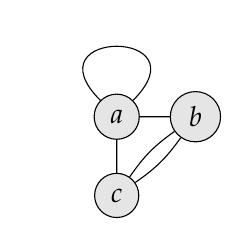
\begin{tikzpicture}
            [main/.style ={draw,circle}]
            \node[main][fill=gray!20!white] (a){$a$};
            \node[main][fill=gray!20!white] (b)[right of = a]{$b$};
            \node[main][fill=gray!20!white](c)[below of= a]{$c$};
            \draw (a) to (b) (c) to (a) (c) to [bend right =10](b) (c) to [bend left =10](b); 
            \draw (a) to [loop,red] (a);
        \end{tikzpicture} 
        \caption{graph $G(V,E)$ is an example of a graphs, the red edge is a loop, and all pair of vertices in this graph is adjecent.}
        \label{fig:graph}
    \end{subfigure}\hfill
   \begin{subfigure}{0.48\textwidth}
    \centering
        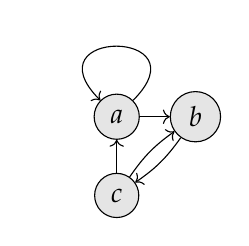
\begin{tikzpicture}
            [main/.style ={draw,circle}]
            \node[main][fill=gray!20!white] (a){$a$};
            \node[main][fill=gray!20!white] (b)[right of = a]{$b$};
            \node[main][fill=gray!20!white](c)[below of= a]{$c$};
            \draw[->] (a) to (b);
            \draw[->](c) to (a);
            \draw[->](c) to [bend left =10](b);
            \draw[->](b) to [bend left =10](c); 
            \draw[->] (a) to [loop,red] (a);
        \end{tikzpicture} 
        \caption{This is an oriantation of the edges in the graph which makes this a digraph}
        \label{fig:digraph}
   \end{subfigure}
\end{figure}


Before delving more specific into graphs and digraphs we must establish some important prerequisite and properties. 
A graph is called \textbf{simple} if there is no loops and no multiple edges. 
With multiple edges it means multiple edges between the same pair of vertices like in \autoref{fig:graph} between $b$ and $c$.
\begin{figure}[!h]
	\centering
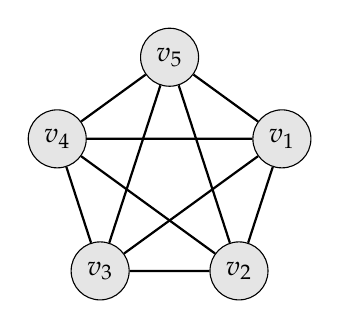
\begin{tikzpicture}[
	xs/.style = {xshift=#1 mm},
	ys/.style = {yshift=#1 mm}]
	
	\def \n {5}
	\def \radius {1.5cm}
	\def \margin {8} % margin in angles, depends on the radius
	
	\foreach \s in {1,...,\n}
	{
		\node[draw, circle][fill=gray!20!white] (\s) at ({360/\n * -(\s+3.75)}:\radius) {$v_\s$};
	}
    \draw[ thick] (1) -- (2) (1) -- (3) (1) -- (4) (1) -- (5);
    \draw[ thick] (2) -- (3) (2) -- (4) (2) -- (5);
    \draw[ thick] (3) -- (4) (3) -- (5);
    \draw[ thick] (4) -- (5);
    \end{tikzpicture}
\caption{Complete graph with 5 vertices.}
\label{fig:complete}
\end{figure}

A graph is \textbf{connected} if there exists a path between all pair of vertices in the graph and \textbf{disconnected} otherwise.
A graph is called \textbf{complete} if there for all pair of vertices in the graph is an edge between them see \autoref{fig:complete}.\\
Somtimes when looking at specifiks set of vertices we are actually interested in something called \textbf{independents set} which is a set of vertices of $G$ where there is no edge between the vertices in the set. A maximal independet set of $G$ is a independent set where you can not add any new vertex in the set that is not adjencent to any vertex in the set(adding a vertex makes the set no longer independent).  
A maximum independent set is the maximal independent set with greatest cardinality. 
Let $I\subset V$ be a maximum independet set then $|I|$ is called the \textbf{independence number}. \\ 

If we instead of edges have \textbf{arcs} between the vertices we call it a \textbf{digraph}.
An arc is describe just like an egde with two adjecent vertices $(a,b)$ the first vertex mentioned in an arc is the vertex \textbf{from} where the arc starts also called the \textbf{tail}, the second vertex is where the arc is pointing \textbf{to} also called \textbf{head}. The set of arcs is normaly denoted $A$ like the set of edges is denoted $E$ 
(so the arc $(a,b)$ goes from $a$ to $b$, if you wanted it the other way around the arc is $(b,a)$).
These graph contaning only arcs and no edges is called a digraph $D(V,A)$ which is what we in this project are focusing on see \autoref{fig:digraph}(as $G$ denote a \textbf{G}raph, $D$ denote a \textbf{D}igraph).\\
For two vertices $x$ and $y$ in $D(V,A)$ then if we have an arc from $x$ to $y$ we say that $x$ \textbf{dominates} $y$ this is denoted like this $x \rightarrow y$. If we talk about subgraphs $A$ and $B$, then $A$ \textbf{dominates} $B$ if for all $a\in A$ and $b\in B$, $a \rightarrow b$. If there is no arcs from $B$ to $A$ we denote it $A\mapsto B$ and if both $A\rightarrow B$ and $A \mapsto B$ we say that $A$ \textbf{completely dominates} $B$ and this is denoted $A\Rightarrow B$.\\ 

Sometimes when working with a digraph or solving a problem we have a subset of vertices $X\subseteq V(D)$ that want to work with as one vertex. 
Then we \textbf{contract} the vertecies $X$ into one vertex $x$ where $N^+(X)\backslash X=N^+(x)$ and $N^-(X)\backslash X=N^-(x)$ (so we only keep the ingoing and outgoing arcs of $X$ and delete all vertices of $X$ and the arcs inside). When we contract $X$ of $D$ we will try uding the notation $D/X$. There is also another kind of contraction where you also delete possible multiple arcs, if this is the case it will be explained in the section.\\

In a digraph we have something called the \textbf{underlying graph} denoted $UG(D)$. 
An underlying graph of a digraph is where all arcs are replaced by edges (edge is used every time we talk about undirected edges between vertices, when using directions it is called an arc).
Let $X \subseteq V$ Then we can make the subdigraph $D\left< X\right>$ which is the subgraph $D$ induced by the set $X$ meaning that all the vertices is from $X$ and the arcs is from $A\in G$ but where both head and tail is incedent to the vertices in $X$. 
We will denote the graph $D\left< V\backslash X\right>$ for some $X\subseteq V$ as $D-X$.
A digraph is \textbf{connected} if the underlying graph is connected, (also called weakly connected), a digraph can be \textbf{strongly connected} and \textbf{semi connected} too.
A digraph is called \textbf{semi connected} if there for each pair $u$ and $v$ exists a path from either $u$ to $v$ or $v$ to $u$.  
It is said to be \textbf{strongly connected} if for each pair of vertices $u$ and $v$ there exists a path from both $u$ to $v$ and $v$ to $u$. A strongly connected digraph is also called a \textbf{strong} digraph. 
A strong digraph have a subset $S$ called a \textbf{seperator} if $D-S$ is not strong, we also say that $S$ \textbf{seperates} $D$. 
A seperator $S$ is called \textbf{minimal seperator} of $D$ if there exists no proper subset $X\subset S$ that seperates $D$.
Now we can introduce a \textbf{$k$-strong} digraph $D$ which is a strong digraph where $|V|> k$ and a minimal seperator $S$ where $|S|= k$.
In the same way we can define $k$\textbf{-arc-strong} digraph is where you need to delete at least $k$ arcs for the digraph to no longer be strong. 

In a digraph $D(V,A)$ we mostly use the \textbf{dregree} as two different degrees namely \textbf{out degree}, $d^+(v)$, and \textbf{in degree}, $d^-(v)$, that is the arcs from $v$ and to $v$ respectively. 
In a digraph $D$ we can talk about the over all \textbf{minimum out degree}, $\delta ^+(D)=\min\lbrace d^+(v)|v\in V\rbrace$ and \textbf{minimum in degree}, $\delta ^-(D)=\min\lbrace d^-(v)|v\in V\rbrace$
somtime we are going to need the minimum of these to $\delta(D)=\min \lbrace\delta ^+(D),\delta ^-(D) \rbrace$ called the \textbf{minimum degree}.
For every vertex $v$ the vertices that is \textbf{adjacent} with $v$ is called \textbf{nieghbours} of $v$.
We denote $N^+(v)$ and $N^-(v)$ as the set of vertices that is dominated by (\textbf{out-nieghbours} of) $v$ and dominates (\textbf{in-nieghbours} of) $v$, respectivly. 
This means that $d^+(v)=|N^+(v)|$ and $d^-(v)=|N^-(v)|$.\\


For simplicity when mentioning paths and cycles in digraphs it will be \textbf{directed} paths and cycles if not anything else is mensioned. 
By \textbf{directed} means that we go from tail to head on every arc on the path or cycle.
When mentioning paths in a digraph it sometimes makes more sence specifing the head an tail of the path, so a path from $s$ to $t$ is denoted as an \textbf{($s,\ t$)-path}.
In some digraphs there is more than one path between the same two vertices these paths can use the same arcs or same vertices or be totally distinct from eachother, the maximum number of disjoint path between two vertices in a digraph is denoted $\lambda_D(s,t)$
 




\section{Computational complexity}
\label{sec:complexity}
In this section we will go over how time is measured for an algorithm and what it means for a problem to be polynomially solveable or polynomially verifyable. Also what it means for a problem to be NP-hard and NP-complete and how we found out if a problem is either of them. 

\subsection{Measure time of algorithm (Polynomial, exponential)}
The runing time of an algorithm is based on how many steps it is going thourgh which is somtimes based on the input that the algorithm takes we are going to denote an algorithms running time as a function $f(n)$ over the input $n$. 
This is how different functions can descirbe the running time of an algorithm, if an algorithm has the same number of steps no matter what the input is it has a constat running time where the constant is the number of steps the algorithm uses. 

An algorithm can also take the form of an polynomial function or even exponentiel, if this is the case we uses some notation as big-$O$ notation or $\theta$. 
Big-oh is the most used one and is the notation we are going to use in this thises, if the algorithm takes $f(n)=4n^3 +2n^2-n+2$ time we denote it in big-oh notation as $O(n^3)$ as it is the biggest term of $f(n)$.  

Since the shorter the runningtime is the better the algortihm is.
Since the exponentiel runningtime algortihms take forever on large inputs, we would want to improve them, but sometimes you are left with problems where that is not a possibility.

So we are going to classify the problems in gruops of how long time it take to decide or verify the problems solution. a problem that is decided i polynomiel time is in the class called $P$.
Which means for every given time of input in a problem from \textbf{P} we can find the solution for the problem in polynomiel time.

\subsection{NP problems and classifications}
As shortly described above there is something called a \textbf{polynomial verifier} for a problem. 
That means given a problem and then given a solution we can in polynomial time verify if it is a solution to the given problem. This is the class we call NP.
\begin{definition}
    \textbf{NP} is the class of languages that have polynomial time verifiers.
\end{definition}

Obiously if you can find a solution in polynomial time you can also verify whether a solution is correct in polynomial time. 
So $P\subseteq NP$. 
There is also a class called $NP-Hard$ but before we can explain that we need to explain what it means for a problem to be polynomial reduceable to another problem. 
For a specific problem $A$ and another problem $B$ then if there exists an algorithm that can take a solution from $A$ and make it a solution for $B$ in polynomial time. 
When such a algorithm exists it is called a polynomial verifier and we say that $A$ is \textbf{polynomial reducable} to $B$ or just that $A$ is \textbf{reduced} to $B$. 
\textbf{NP-Hard} are the class of problems that every NP problem can be polynomiel reduced to. 
A problems in the class of NP-Hard problems does not nessesarily mean that it is NP it-self.
If a problem is both \textbf{NP} and \textbf{NP-Hard} we call it \textbf{NP-Complete}. 
The problems we are \textcolor{red}{mostly} focusing on is in the class of \textbf{NP-Complete} problems.
   

\section{Classes of Digraphs}
\label{sec:class}
We can classefy specific collection of graphs the reason for this is that digraphs of smaller collections of digraphs (like tournaments is a smaller collection of semicomplete digraphs) might be because of problems that is hard to solve on general digraph but is \\
easy/polynomial solvable on specific types of digraphs.

A group of these problems is called NP-complete problems which sometimes sound easy solvable for graphs but only for some specific graphs we know how to solve it in polynomial time. 
Like finding paths in digraphs or cycles or more specific things, but in general des more we know about a digraph we can use to solve hard problems which in general would be time consuming like the problems that are NP-hard.
By some quick fast algorithm you can checks wheter a digraph belongs to a certion \textbf{class} of digraphs. 
A class of digraph is a collection of digraph with certain properties incommen like \textbf{tournaments}.\\
\subsection{introduction to some digraph classes}
\textbf{Tournaments} is a digraph where the underlying graph is complete. 
So a complete graph of order 5 any orientation of the edges concludes in a tournament.
Strong digraphs is also in it self a classification of digraphs. Classes of digraphs can be overlapping each other or be fully containt in each other like tournaments is fully containt in the class called semicomplete digraph.
A \textbf{semicomplete} digraph is where the underlying graph is complete multigraph, there can be some multiple edges in between the same pair of vertices in the underlying graph. Since the class called semicomplete digraphs contains all digraphs where the underlying graph is a complete multigraph it clearly also contains the graph with only one arc between every pair of vertecies (Tournaments).
A \textbf{complete} digraph is where every pair of vertices $a,b\in V$ the arc $(a,b)$ and $(b,a)$ is present in the graph. \\
If you can split the graph into two sets of vertices $A$ and $B$ such that $A\cup B=V$ and there is no arcs inside these sets, then we classify this as an \textbf{bipartite} digraph This means all arcs in the graph is in the form $(a,b)$ or $(b,a)$ for all $a\in A$ and $b\in B$. 
The sets $A$ and $B$ are called the partites of $D(V,A)$. 
The underlying graph of a bipartite digraph is also called bipartite since there is no edges inside $A$ or $B$.
If there exists more then two of these partite sets we call the digraphs \textbf{multipartite}, since there is multiple partite sets in the graph, bipartite sets $\subset$ multipartite. \\
A much used type of digraph is an \textbf{acyclic} digraph. 
It is a digraph where for an specific ordering of the vertices $V={v_1, v_2,\dots , v_n}$ the arcs in the digraph is $(v_i, v_j)$ where $i<j$ for all $(v_i, v_j)\in A$. This ordering is called an \textbf{acyclic ordering} and can also be used to order strong components in an non-strong digraph such that the ordering of the componentent $C_1,C_2,\dots C_k$ is an acyclic digraph when contracting the components into $k$ vertices. 
When classifying digraphs there is several ways of doing this, like \textbf{transitive} digraphs which are digraphs where for all vertices $a,d,c\in V$ where the arc $(a,b)$ and $b,c$ is present in the digraph ($\in A$), the arc $(a,c)$ has to be a part of $A$ too. 
using the same kind of classification there is digraphs which are \textbf{Quasi-transitive} which is forall vertices $a,d,c\in V$ where the arc $(a,b)$ and $b,c$ is present in the digraph ($\in A$), $a$ and $c$ has to be adecent by at \textit{least} one (more arcs in between are also allowed) arc in either direction ($(a,c)$ or $(c,a)$). These graphs are going to be mentioned a lot in this thises since the graph is also what we call \textbf{decomposable}.\\
\textbf{Decomposable} digraphs is also a clasification of graphs which are decomposable, for a graph $D$ to be decomposable we have $H_1,H_2, \dots , H_k$ \textbf{houses} and $S$ where $V(S)={s_1,s_2,\dots,s_k}$ which are all digraphs by them self but if each $s_i$ is replaced by the digraph $H_i$ $i=1,2,\dots,k$ we have the graph $D$, where $H_i\rightarrow H_j \in D$ if $s_i\rightarrow s_j\in S$  denote this decomposition like $D=S[H_1,H_2,\dots H_k]$.
This is the class of digraphs we are focusing on in this thises. 
If all the houses are independent sets we call $D=S[H_1,H_2,\dots ,H_k]$ the extension of $S$. 
If $S$ is a semicomplete digraph we call the extensin of these \textbf{extended semicomplete} digraph.
Like we already mentioned Quasi-transitive digraphs are decomposable but we have several classes that are decomposable, and another class of digraphs that is giong to be used a lot in this is \textbf{locally semicomplete} digraphs.\\
First we are going to introduce \textbf{in-locally semicomplete} digraphs and \textbf{out-locally semicomplete} digraphs which is for every in-nieghboor of a vertex $x\in V$ they have to be adjecent ($x\cup N^-(x)$ induces a semicomplete digraph) is the in-locally semicomplete digraph if it is true for all $x\in V$. 
Respectively it is called an out-locally semicomplete digraph if $\forall x\in V$ the out-nieghboors, $N^+(x)$, has to be adjecent. 
If a digraph is both in-locally semicomplete and out-locally semicomplete, it is called a \textbf{locally semicomplete} digraph. Why both Quasi transitive digraphs and some locally semicomplete digraphs are decomposeble will be described in section \autoref{sec:Decomposable}.\\
The last class of digraph that are important for this thises is the round digrphs. 
A digraph is called a \textbf{round} digraph if there exists an ordering of the vertices $v_1,v_2,\dots,v_n$ such that for all $v_i$, $N^+(v_i)={v_{i+1},v_{i+2},\dots ,v_{i+d^+(v_i)}}$ and $N^-(v_i)={v_{i-d^-(v_i)},v_{i-(d^-(v_i)-1)},\dots ,v_{i-1}}$.






\chapter{Decomposable Digraphs}
\label{chap:decomposable}
Decomposable digraphs is what we in this thesis is focusing on. 
We have introduced short what a decomposable digraph is but there is subclasses to focus on and a lot of other crucial definitions and theroems to cover about these digraphs before delving into the NP-hard problems. 
First we cover some general things about decomposable digraphs the next section is about quasi-transitive digraphs, and why they are a subclass of decomposable digraphs and $\phi_1$-decomposable digraphs. At the end of the section we prove that these decompositions can be found in polynomial time. 
Which is going to be crucial for solving some NP-hard problems for this class of digraphs. Then we are going to look at a very general class of digraphs locally semicomplete digraphs, where this class can be split up to 3 different subclasses where 2 of those are decomposable. 
This is covered in \autoref{sec:locally} and is going to be used in later chapthers. 
\section{General about Decomposable digraphs}
\label{sec:gdecomposable}
Recall that a decomposable digraph $D$ can be decomposed into a main graph $S$ where $|S|=k$ and $k$ houses $H_1,H_2,\dots , H_k$, where each vertex in $S=\lbrace v_1,v_2\dots ,v_k\rbrace$ is replaced by the house $H_i$ replace $v_i$ and the arcs between the houses is as follows $H_i \rightarrow H_j$ in $D$ if $v_i\rightarrow v_j$ in $S$ remember that for a set $X$ to dominate an other set $Y$ (meaning every vertex in the dominating set dominates every vertex in the dominated set) we denoted it $X \rightarrow Y$. If no arc between $v_a$ and $v_b$ in $S$ then there is no arc between the sets $H_a$ and $H_b$ in $D$. 
The thing about decomposable digraphs is that if there is an arc between $H_i$ and $H_j$ either one of the houses totally dominates the other (ex. $H_i \Rightarrow H_j$) or they dominate each other (ex. $H_i \rightarrow H_j$ and $H_j\rightarrow H_i$).

Decomposable digraphs can be classed by a set of digraphs $\phi$, when \\
$D=S[H_1,H_2,\dots ,H_k]$ it is \textbf{$\phi$-decomposable} if $D\in \phi$ or if $S\in \phi$. The chioces of $H_i$ for $i=1,2\dots , k$ does not determine anything about the digraph being $\phi$-decomposable but the class of \textbf{totally $\phi$-decomposable} digraphs is where $D$ is $\phi$-decomposable and each $H_i$ is totally $\phi$-decomposable. 
We are going to make two shuch sets of digraphs $\phi_1$ which is the union of semicomplete digraph and acyclic digraph both classes deskribed in \autoref{sec:class} and $\phi_2$ which is the union of semicomplete and round digraphs also deskribed in \autoref{sec:class}.  
\begin{align}
    \phi_1=\text{Semicomplete digraphs}\cup \text{Acyclic digraphs}
    \label{eq:phi1}\\
    \phi_2=\text{Semicomplete digraphs}\cup \text{Round Digraphs}
    \label{eq:phi2}
\end{align}

\section{Quasi-transitive Digraph}
\label{sec:quasi}
First we need to recall what a quasi transitive digraph is. 
For every triplet $x,y,z$ in a quasi-transitive digraph if $x\rightarrow y$ ($x$ dominates $y$) and $y\rightarrow z$ ($y$ domitaes $z$), then there has to be at least one arc in either dirction between $x$ and $z$. 
When working with quasi-transitive digraphs there are many things you can depend on, things that the structure has already diceded for us.
\begin{lemma}~\cite{banggutin}
    Suppose that $A$ and $B$ are distinct strong components of a quasi-transitive digraph $D$ with at least one arc from $A$ to $B$. Then $A\rightarrow B$.
    \label{lemma:dominatingset}
\end{lemma}
Recall that this means that every vertex in $A$ has an arc to every vertex in $B$.
Like non-strong quasi-transitive digraph we can also say something about strong quasitransitive digraphs.
\begin{lemma}~\cite{banggutin,bangJGT2}
    Let $D$ be a strong quasi-transitive digraph on at least two vertices. Then the following hold:
    \begin{itemize}
        \item[(a)] $\overline{UG(D)}$ is disconnected;
        \item[(b)] If $S$ and $S'$ are two subdigraphs of $D$ such that $\overline{UG(S)}$ and $\overline{UG(S')}$ are distinct connected components of $\overline{UG(D)}$, then either $S\rightarrow S'$ or $S'\rightarrow S$ or both $S\rightarrow S'$ and $S'\rightarrow S$ in which case $|V(S)|=|V(S')|=1$. 
    \end{itemize} 
    \label{lemma:underlyinggraph}
\end{lemma}
These to lemmas is also a part of proving the one theorem which states that quasi-transitive digraphs can be decomposed no matter if there are strong or nonstrong digraphs. 

\begin{thm}\cite{bangJGT85}
    Let $D$ be a quasi-transitive digraph.
    \begin{enumerate}
        \item If $D$ is not strong, then there exists a transitive acyclic digraph $T$ on $t$ vertices and strong quasitransitive digraphs $H_1,\dots,H_t$ such that $D=T[H_1,\dots,H_t]$.
        \item If $D$ is strong, then there exists a strong semicomplete digraph $S$ on $s$ vertices and quasitransitive digraphs $Q_1,\dots ,Q_s$ such that each $Q_i$ is either a single vertex or is nonstrong and $D=S[Q_1,\dots,Q_s]$.
    \end{enumerate}
    \label{thm:quasidecom}
\end{thm}
This theroem is also what we are going to use more then ones, to prove several of the problem solving theorems through out this thises.
\begin{proof}
    Since we can decompose both strong quasi-transitive digraphs and non-strong quasi-transitive digraph we are going to prove if $D$ is not strong first and there after if $D$ is strong.
    So suppose $D$ is not strong, then we know we can enumerate the strong components in an acyclic order let these be $H_1,\dots , H_t$. \\
    Recall that an acyclic ordering of the strong components does not mean that there is no arcs going back in the ordering, but we will prove that now. \\
    Now from \autoref{lemma:dominatingset} we know that if there is an arc between two of the strong components, one of them dominates the other.
    Let with out loss of generality these set be $H_i$ and $H_j$ and let $H_i\rightarrow H_j$. 
    Then Since $D$ is not-strong $H_j\nrightarrow H_i$ now let say that $H_j \rightarrow H_k$, then since $D$ is quasi-transitive then either $H_k\rightarrow H_i$ or $H_i \rightarrow H_k$. 
    But since $H_i\cup H_j \cup H_k$ is not strong $H_k\nrightarrow H_i$ meaning contracting each $H_i$ for $i=1\dots,t$ we will have a transitive digraph $T$ and we have also shown that there are no backwards going arcs in the ordering meaning that $T$ is not only transitive but acyclic. 
    This end the proof of the non-strong quasi-transitive digraph leving only the strong ones left.\\

    Now suppose that $D$ is a strong quasi-transitive digraph, we now look at the underlying graph $UG(D)$ after this we find the complement of it, $\overline{UG(D)}$ since $D$ is strong we know from \autoref{lemma:underlyinggraph} that $\overline{UG(D)}$ is disconnected, so we find $Q_1,\dots , Q_s$ where $\overline{UG(Q_i)}$ is connected in $\overline{UG(D)}$ $\forall i \in [s]$.\\ 
    Since these subdigraphs $\overline{UG(Q_i)}$ of $\overline{UG(D)}$ is connected we know that $Q_i$ is non-strong or a single vertex in $D$. 
    From the same lemma each $Q_i$ (reprecent $S$ in \autoref{lemma:underlyinggraph}) which means when contracting $Q_i$ $\forall i\in [s]$ into a single vertex $q_i$. 
    Denote $D$ with contracted $Q_i$'s as $S$. 
    We have that every pair of vertex in $S$ have one arc between in either direction or one in both direction making $S$ semicomplte. \\
    This concludes the proof.
\end{proof}
From this theorem we can see that quasi-transitive digraphs is totally $\phi_1$-decomposable. 
Since the transitive digraph for the nonstrong quasi-transitive digraphs is acyclic $T\in \phi_1$ and each $H_i$ is itself strong quasi-triansitive digraphs and you can therefore use \autoref{thm:quasidecom} agian.  
For the strong quasi-transitive digraphs $D$, $S$ is semicomplete so $S\in \phi_1$ and each $Q_i \in \phi_1$ because it is either one vertex which is a digraph that is both acyclic and semicomplete or it is non-strong and must be quasi-transitive and therefore \autoref{thm:quasidecom} can be used agian. So every nonstrong and strong quasi-transitive digraphs is totally $\phi_1$-decomposable.

\begin{thm}
    \textcolor{red}{quasi decomposition can be found in poly time}
\end{thm}

\section{Locally semicomplete Digraph}
\label{sec:locally}
blablabla
\begin{thm}
    \textcolor{red}{round decompose locally semicomplete digraph}
\end{thm}
Every locally semicomplete digraph can be classified into some other groups of digraphs namely semicomplete digraphs and round decomposable digraphs and the last one which is neither of the two is call evil. Round decomposable digraph $D=R[D_1,\dots,D_r]$ is where $R$ is a round digraph of the strong componentents $D_i$ and $|R|=r$.
\begin{thm}~\cite{bangJGT85}
    Let $D$ be a locally semicomplete digraph. Then exactly one of the following possibilities holds. Furthermore, there is a polynomial algorithm that decides which of the properties hold and gives a certificate for this.
    \begin{itemize}
        \item[(a)] $D$ is round decomposable with a unique round decomposition $R[D_1,\dots ,D_r]$, where $R$ is a round local tournament on $r\geq 2$vertices and $D_i$ is strong semicomplete digraph for $i=1,2,\dots,r$.
        \item[(b)] $D$ is evil 
        \item[(c)] $D$ is a semicomplete digraph thet is not round decomposable. 
    \end{itemize}
\end{thm}
If the locally semicomplete digraph is nonstrong it turns out that it is decomposable this is called a semicomplete decomposition.
\begin{thm}~\cite{bangJGT85,banggutin,bangJCT102}
    Let $D$ be a nonstrong locally semicomplete digraph and let $D_1,D_2,\dots,D_p$ be the acyclic order of the strong components of $D$. Then $D$ can be decomposed into $r\geq 2$ disjoint subdigraphs $D_1',D_2',\dots, D_r'$ as follows:
    \begin{align*}
        D_1'=D_p, \lambda_1=p,\\
        \lambda_{i+1}=min\lbrace j|N^+(D_j)\cap V(D'_i)\neq \emptyset\rbrace,
    \end{align*}
    and
    \begin{equation*}
        D'_{i+1}=D\left<V(D_{lambda_{i+1}})\cup V(D_{lambda_{i+1}+1})\cup \cdots \cup V(D_{lambda_{i}-1})\right>
    \end{equation*}
    The subdigraphs $D'_1,D'_2,\dots,D'_r$ satisfy the properties below:
    \begin{itemize}
        \item[(a)] $D'_i$ consists of some strong components that are consecutive in the acyclic ordering of the strong components of $D$ and is semicomplete for $1=1,2,\dots,r$;
        \item[(b)] $D'_{i+1}$ dominates the initial component of $D'_i$ and there exists no arc from $D'_i$ to $D'_{i+1}$ for $i=1,2,\dots,r-1$;
        \item[(c)] if $r\geq 3$ then there exists no arc between $D'_i$ and $D'_j$ for $i,j$ satisfying $|j-i|\geq 2$  
    \end{itemize}
    \label{thm:semicompletedecom}
\end{thm}
For simplification of \autoref{thm:semicompletedecom} the properties is drawn out in \autoref{fig:properties}
\begin{figure}
    \begin{tikzpicture}
        \node[$a$](a)
    \end{tikzpicture}
    \caption{(a)(b) and (c)}
    \label{fig:properties}
\end{figure}
Now we focus more on the structure of the evil locally semicomplete digraph which we have not covered jet, there is a fine understanding of the structure of round decomposable and the semicomplete digraphs, even the semicomplete decomposition which is a part of the evil structure too.
First we have to recall what a minimal seperator from \autoref{sec:digraph}, then use this to construct what we call a \textbf{good} seperator.
\begin{lemma}~\cite{bangJGT85}
    Let $S$ ba a minimal seperator of the locally semicomplete digraph $D$. Then either $D\left< S\right>$ is semicomplete or $D\left< V-S\right>$ is semicomplete.
    \label{lem:whichsemicomplete}
\end{lemma}
Then a \textbf{good} seperator of a locally semicomplete digraph is minimal and $D\left<V-S\right>$ is not semicomplete.
When finding a good seperator in a evil locally semicomplete digraph, then the part that is left $D-S$ a semicomplete decomposition can be found it turns out that there is a lot to say about this decomposition.
\begin{thm}~\cite{bangJGT85,bangJCT102}
    Let $D$ be an evil locally semicomplete digraph then $D$ is strong and satisfies the following properties.
    \begin{itemize}
        \item[(a)]There is a good seperator S such that the semicomplete decomposition of $D-S$ has exactly three components $D'_1,D'_2,D'_3$ (and $D\left<S\right>$ is semicomplete by \autoref{lem:whichsemicomplete});
        \item[(b)] Furthermore, for each such $S$, there are integers $\alpha, \beta,\mu,\nu$ with $\lambda_2\leg \alpha \leq \beta \leq p-1$ and $p+1\leq \mu \leq \nu \leq p+q$ such that 
        \begin{align}
            &N^-(D_\alpha)\cap V(D_\mu)\neq \emptyset \text{and} N^+(D_\alpha)\cap V(D_\nu)\neq \emptyset,\\
            \text{or} &N^-(D_\mu)\cap V(D_\alpha)\neq \emptyset \text{and} N^+(D_\mu)\cap V(D_\beta)\neq \emptyset,
        \end{align} 
        where $D_1,D_2,\dots, D_p$ and $D_{p+1},\dots,D_{p+q}$ are the strong decomposition of $D-S$ and $D\left< S\right>$, respectively, and $D_{\lambda_2}$is the initial component of $D'_2$ 
    \end{itemize}
    \label{thm:evildecom}
\end{thm}
Even though this is a structure we can work with, we can actually go deeper into the structure of this evil locally semicomplete digraph. Namly trying to group the components inside the semicomplete decomposition $D'_1,D'_2,D'_3$ and the good seperator $S$. This structer is menation in \cite{bangJGT85} but also in \cite{tildeDMCS}. First we can establish this lemma which is a big part of the structure of evil locally semicomplete digraphs.
\begin{lemma}~\cite{tildeDMCS}
    Let $D$ be an evil locally semicomplete digraph and let $S$ be a good seperator od $D$. Then the following holds:
    \begin{itemize}
        \item[(i)] $D_p\Rightarrow S\Rightarrow D_1$.
        \item[(ii)] If $sv$ is an arc from $S$ to $D'_2$ with $s\in V(D_i)$ and $v\in V(D_j)$, then 
        \begin{equation*}
            D_i\cup D_{i+1}\cup \dots D_{p+q}\Rightarrow D_1\cup\dots \cup D_{\lambda_2-1}\Rightarrow D_\lambda_2\cup \dots \cup D_j
        \end{equation*}.
        \item[(iii)] $D_{p+q}\Rightarrow D'_3$ and $D_f\Rightarrow D_{f+1}$ for $f\in [p+q]$, where $p+q+1=1$.
        \item[(iv)] If there is any arc from $D_i$ to $D_j$ with $i\in [\lambda_2-1]$ and $j\in [\lambda_2,p-1]$, then $D_a\Rightarrow D_b$ for all $a\in [i,\lambda_2-1]$ and $b\in[\lambda_2,j]$.
        \item[(v)] If there is any arc from $D_k to D_l$ with $k\in [p+1,p+q]$ and $l\in [\lambda_2-1]$, then $D_a\Rightarrow D_b$ for all $a\in [k,p+q]$ and $b\in [l]$.   
    \end{itemize}
\end{lemma}


\chapter{Path cover and hamilton cycles}
\label{chap:hamilton}
In this chapter the focus is the hamilton cycle problem, where we know that if we can solve the path covering problem then we can solve the hamilton cycle problem for quasi-transitive digraphs.\\
In the first section we are going to cover, what a hamilton path is, and a hamilton cycle Since these to problems are well know as \textbf{NP-Complete} which will shortly be introduced too.\\
The next section is about path-mergeable digraphs and that locally semicomplete digraphs are a subclass of these and how this helps in the path covering problem and hamilton cycle problem. 
%Then state some theorems that says knowing special things about the graph we know when it contain a hamilton cycle. \\
The following section is covering quasi-transitive digraphs and whether or not there exists a hamilton cycle in those. Here the decomposition of the quasi-transitive digraphs is going to be a crucial part of proving this. \\


\section{The Hamilton Path and Cycle Problem}
\label{sec:hNP}
Finding a hamilton cycle in a digraph is a well know problem, but here is a shortly explanaition of what that is.
When we define what a hamiltonian digraph is we first have to explain what a hamilton cycle is. A hamilton cycle is a directed cycle $C_H$ in a digraph that contains(pass by) every vertex in the digraph $\forall v\in V(D), v$ is in $C_H$.\\
\begin{definition}
    A Hamiltonian digraph is a graph containing a hamilton cycle 
\end{definition} 
We can also define digraphs called traceable
\begin{definition}
    A traceable digraph is a digraph containing a hamilton path
\end{definition}
A hamilton path is a path containing all vertices of the digraph.\\
The problems that is considered \textcolor{red}{NP-Hard} is finding out whether an arbitrary digraph is trecable or hamiltonian. 
We are going to show that hamilton cycle problem is \textcolor{red}{NP-Hard} by reducing it to a problem we know is. 
Then we are going to show that if we know that a digraph is traceable it takes polynomial time to figure out wheter it is hamiltonian too, making the traceable problem \textcolor{red}{NP-Hard} too. 
Because if the you in polynomial time could figure out wheter a arbitrary digraph is traceable you know that if it is not, it is defenatly not hamiltonian. 
And if it is you can in polynomial time figure out if it is hamiltonian, making the hamton cycle problem a polynomial time solution problem (not \textcolor{red}{NP-Hard}). 
\section{Hamiltonian Locally semicomplete Digraphs}
\label{sec:hlocally}
Recall that a locally semicomplete digraph is both in-locally semicomplete and out-locally semicomplete. 
Before this gets relevant we are going to introduce a class of digraphs called path-mergeable they are not introduced under section \autoref{sec:class} since we are only going to use it in this section.
A short explanaition of a path mergeable digraph is that it is the class of digraphs where given two paths with the start- and endpoint incommen you can merge the two paths into one using all vertices in the two paths. 
A more formal definition of path mergeable digraphs is if there exists a pair of distinct vertices $x,y\in V(D)$ and any two disjoint $(x,y)$-paths there exists a new path from $x$ to $y$ where it is a union of the vertices used in the two vertex-disjoint paths (ending up with a "merge" path of the two given path).\\
These digraphs are easy to regonize with the following corolary we can do it in polynomial time too and the following theroem gives us a nice propertie of path-mergeable digraphs.
\begin{cor}~\cite{banggutin}
    Path-mergeable digraphs can be regonized in polynomial time
\end{cor}
\begin{thm}~\cite{banggutin}
    A digraph $D$ is path mergeable if and only if for every pair of distict vertices $x,y\in V(D)$ and every pair $P=xx_1\dots x_ry,\ P'=xy_1\dots y_sy$, $r,s\geq 1$ of internally disjoint $(x,y)$-paths in $D$, either there exists an $i\in \lbrace 1,\dots ,r\rbrace$, such that $x_i\rightarrow y_1$, or there exists a $j\in \lbrace 1,\dots, y_j\rightarrow x_1\rbrace$.
    \label{thm:pathmerge}
\end{thm}
to explain this \autoref{thm:pathmerge} it tells us that for every path mergeable digraph in every two disjoint $(x,y)$-path there has to be from one of the path a vertex that dominates the first vertex after $x$ in the other path. This has to hold for every distict pair of vertices $x$ and $y$. \\
It turns out that in these digraph we can easily determine whether it is a hamiltonian digraph too.
\begin{thm}
    A path-mergeable digraph $D$ of order $n\geq 2$ is hamiltonian if and only if $D$ is strong and $UG(D)$ is $2$-connected.
    \label{thm:pathham}
\end{thm}
\begin{cor}
    There is an $O(nm)$-algorithm to decide whether a given strong path-mergeable digraph has a hamiltonian cycle and find one if it exists.
    \label{cor:polypath}
\end{cor}
So it turns out that for path-mergeable digraphs this problem is polynomial solveable, and a subclass of these path-mergeable digraph is namely the locally semicomplete digraphs. If we can prove this we only know that we can solve the hamilton cycle in polynomial time and since the locally semicomplete digraphs is a subclass of in-locally semicomplete digraphs we have an even better time for these.
\begin{prop}
    Every locally in-semicomplete (out-semicomplete) digraph is path-mergeable.
\end{prop}
\begin{proof}
    proof this ... ... ... ... ... ... ... 
\end{proof}

Then it turns out that \autoref{thm:pathham} and \autoref{cor:polypath} can be imporved if we are only looking at the in-locally semicomplete digraph, since the locally semicomplete digraph is a subclass of these, and it is the ones we are interested in, in this thises. It turns out that every strong in-locally semicomplete digraph has a 2-connected underlyning graph, which means the only thing we need to check is whether it is a strong digraph.
\begin{thm}
    A locally in-semicomplete digraph $D$ of order $n\geq 2$ is hamiltonian if and only if $D$ is strong.
\end{thm}

It turns out that when looking at the strong locally in-semicomplete digraphs out of the path-mergeable digraph finding the hamiltonian cycle can be done i polynomial time by theorem discorvered by ... ...
\begin{thm}
    There is an $O(m+n\text{log}n)$-algorithm for finding a hamiltonian cycle in a strong locally in-semicomplete digraph.
\end{thm}


\section{Hamiltonian Quasi-transitive Digraphs}
\label{sec:hquasi}
First of all we have to recall \autoref{thm:quasidecom} since it is the key theorem to solve the hamiltonian problem in polynomial time. \\
Remember that a condition for a digraph to be hamiltonian is that it need to be strong, so for finding a hamilton cycle in a quasi-transitive digraph, we are not interested in the non-strong digraphs. 
Leving only the strong quasi-transitive digraphs with decomposition $S[Q_1,\dots Q_s]$ from \autoref{thm:quasidecom}. 
The given decomposition of strong quasi-transitive digraphs has a semicomplete digraph as the quotient. This is why we need some inside to these before the main solution in this subsection can be proven. another composition of semicomplete digraphs is the extension of these, called extended semicomplete digraph. An extension of a digraph is a composition of the given digraph $S$ where the hauses of the composition is either a single vertex or independence sets. \\
Before we explain when we can find a hamilton cycle in strong quasi-transitive digraphs we need to recall what a cycle factor is. 
From \autoref{sec:digraph} we shortly explain that a cycle factor is when we can find $C_1,\dots C_k$ cycles in $D$ contaning all vertices of $D$. 
\begin{thm}~\cite{gutinMNN2}
    An extended semicomplete digraph $D$ is hamiltonian if and only if $D$ is strong and contains a cycle factor. One can check whether $D$ is hamiltonian and construct a Hamilton cycle of $D$ (if one exsists) in time $O(n^{2.5})$.
    \label{thm:extended}
\end{thm}
\begin{thm}~\cite{bangJGT20}
    A strong quasi-transitive digraph $D$ with a canonical decomposition \\$D=S[Q_1\dots, Q_s]$ is hamiltonian if and only if it has a cycle factor $\mathcal{F}$ such that no cycle of $\mathcal{F}$ is a cycle of some $Q_i$.
    \label{thm:qhcycle}
\end{thm}
\begin{proof}
    Since a hamiltonian cycle need to cover all vertices in a digraph, we know that it must cross every $Q_i$. 
    Moreover the hamilton cycle is a cycle factor not fully containt in any $Q_i$. So we only need to show that if we have a cycle factor $\mathcal{F}$, where no cycle is in any $Q_i$, then $D$ is hamiltonian. $\forall i$ $V(Q_i)\cap \mathcal{F}=\mathcal{F}_i$, there can not be any circle in this and since every vertex is in $\mathcal{F}$ all vertices in $Q_i$ must be containt in $\mathcal{F}_i$ and there is no cycle containt in $\mathcal{F}_i$ whcich makes it a path factor of $Q_i$.\\
    \textcolor{red}{Figure here}\\
    For all paths in $\mathcal{F}_i$ we make a path contraction. 
    After contraction or before we delete the remaining arcs if this is done before its the arcs going from the end of a path to a begining of an other path. This action will make $Q_i$ an independent set $\forall i\in [s]$. Since $S$ is a semicomplete digraph our new digraph would then because of the independence of each $Q_i$ after the action be an extended semicomplete digraph $S'$. 
    Since we have only made path contractions along the cycles in the cycle factor of $D$ and not deleted any arcs that are a part of the cycle factor $S'$ contains a cycle factor. 
    Then by \autoref{thm:extended} we know that $S'$ contains a hamilton cycle. Adding the deleted arcs does not change this insert a path instead of a node just makes the cycle longer but it still contains every vertex given a hamilton cycle in $D$
\end{proof}

A hamilton path does not have the same condition for a digraphs to be strong meaning we are also interested in the non-strong quasi-transitive digraphs $T[H_1,\dots ,H_t]$. 
The next theorem is proven in much the same as \autoref{thm:qhcycle}. 
\begin{thm}~\cite{bangJGT20}
    A quasi-transitive digraph $D$ with at least two vertices and with canonical decomposition $D=R[G_1,G_2,\dots , G_r]$ is traceable if and only if it has a $1$-path-cycle factor $\mathcal{F}$ such that no cycle or path of $\mathcal{F}$is completely in some $D\left< V(G_i)\right>$.
\end{thm}

We know that the canonical decomposition of a quasi-transitive digraph can be found i polynomial time. 
We can also find the hamilton cycle in a quasi-transitive digraph in polynomial time, but also verify if it does not exists for the given graph. This result was proved by Gutin. ... 

\begin{thm}~\cite{banggutin94}
    There is an $O(n^4)$ algorithm which, given a quasi-transitive digraph $D$, either returns a hamiltonian cycle in $D$ or verifies that no such cycle exists.
\end{thm}






	\clearpage
	\part{Linkage and Weak Linkage}
	\chapter{Disjoint path in decomposable digraphs}
\label{chap:linkage}
In this chapter we will cover the Linkage problem given a set a decomposable digraph $D$ and a set of terminals $\Pi$ to be linked. 
We will explaining the problem and shortly show why the problem is interresting (NP-complete). 
After this we will in \autoref{sec:lQuasi} show that the linkage problem is polynomial solveable in $\phi$-decomposable digraph as long as $\phi$ is a linkage ejector after that we will show that $\phi_1$ is a linkeage ejector meaning that the linkage problem is solveable for quasi-transitive digraphs(all of this is only true if the number of pairs needed linking is fixed). Then in \autoref{sec:lLocally} we will cover the 3 different subclasses a locally semicomplete digraph can be a part of, and solve the $k$-linkage problem for those in polynomial time for a fixed $k$. 
\section{The Linkage Problem}
\label{sec:lNP}
Given a digraph $D$ and two distinct vertices $s$ and $t$ we want to make a path from $s$ to $t$ denoted this $P$. 
Recall that in this case $s$ will be the source of $P$ and $t$ the zink.
This we sould be able to do easily if one exists, but when adding two extra distict vertices $u$ and $v$ not nessesarily distinct from $s$ and $t$ and we want a path $Q$ between $u$ and $v$ distinct from the path $P$ the problem suddenly become NP-complete.
This prolem is what we call the \textbf{2-linkage} problem, we can replace 2 with an arbitrary number $k$ and we then call it the \textbf{$k$-linkage} problem or just \textbf{the linkage problem}. 
the vertices $s$, $t$, $u$ and $v$ are called \textbf{terminals} and $(s,t)$, $(u,v)$ are called \textbf{terminal pairs}.
\begin{thm}
    \textcolor{red}{linkage NP-complete}
\end{thm}
\begin{proof}[skezt]
    \textcolor{red}{blblablbalablablabala}
\end{proof}
The notation for this problem in this thesis would be using $k$ as the natruel number of pairs of terminals, and the set of these terminals is denoted $\Pi=\lbrace (s_1,t_1);\dots ;(s_k,t_k)\rbrace$. 
As we have done optil now we will still use $D$ as the main digraph we are looking at unless anything else is specified. 
$L$ is used as a colloction of paths $P_1,\dots , P_l$ if $L$ is the solution to our linkage problem it means $l=k$ and and the paths $P_i$ links the pair $(s_i,t_i)$ for all $i\in [k]$.
If $L$ upholds the above conditions we say that $L$ is a $\Pi$-linkgae, or $L$ is the linkage of $(D,\Pi)$.\\
Recall that a quasi-transitive digraph is build up by either a transitive acyclic digraph or semicomplete digraph as the quotient of the decomposition. 
And for these to classes of digraph we kan solve the $k$-linkage problem in polynomial time for a fixed $k$. With fixed $k$ there means that an algorithm given a digraph and a naturel number $k$ can solve the $k$-linkage problem(it is possible that the algorithm needs more information). When $k$ is not fixed then it is already NP-complete for tournaments, since tournaments is a very strict class we will only focus on when $k$ is fixed.


\section{Solving the Linkage Problem in $\phi$-decomposable Digraphs}
\label{sec:lQuasi}
From \autoref{thm:quasidecom} we know that a quasi-transitive digraph is a composition of acyclic transitive digraphs and semicomplete digraphs.
We know that $\phi_1$ is the union of acyclic and semicomplete digraphs, which means that every quasi-transitive digraphs are $\phi_1$-decomposable as described in \autoref{chap:decomposable}. 
\begin{thm}~\cite{bangJGT85}
    For every fixed $k$, there exists a polynomial algorithm for the $k$-linkage problem on acyclic digraphs.
    \label{thm:acyclicklink}
\end{thm}
\begin{thm}~\cite{chudnovskyAM270}
    For every fixed $k$, there exists a polynomial algorithm for the $k$-linkage problem on semicomplete digraphs.
    \label{thm:semiklink}
\end{thm}
Note that this means that there exists polynomial algorithms for a fixed $k$ to solve the $k$-linkage problem for digraphs in $\phi_1$.\\
For a decomposition $D=S[M_1,\dots M_s]$ and a set of terminal pairs, we can split the set into two different sets of terminals. 
The set of \textbf{internal pairs} $\Pi_i$, where internal pair means that both $s_i$ and $t_i$ is in the same house, and the set of \textbf{external pairs} $\Pi_e$ which is the rest such that $\Pi=\Pi_i \cup \Pi_e$.\\
\begin{lemma}~\cite{bangJGT85}
    Let $D=S[M_1,\dots ,M_s]$ be a decomposable digraph and $\Pi$ a set of pairs of terminals. Then $(D,\Pi)$ has a linkage if and only if it has a linkage whose external paths do not use any arc of $D\left<M_i\right>$ for $i\in [s]$.
    \label{lemma:externalhouse}
\end{lemma}
\begin{proof}
    One direction is trivial since a linkage where external paths uses no arcs inside any house is still a $(D,\Pi)$-linkage.
    So now we assume that $L$ is a $(D,\Pi)$-linkage that uses the smallest amount of vertices possible. 
    We claim that no external path of $L$ uses any arcs inside any house. 
    Now we assume that this is not the case, then there must exist a path $P\in L$ where an arc $uv$ of $P$ is \textcolor{red}{containt in} a house $uv\in A(P)\cap A(D\left<M_i\right>)$ for some $u,v\in V(P)$ and some $i\in [s]$.\\
    Since $P$ is external there is at least one vertex outside the house, ($z\in V(P)-V(M_i)$) either $zu$ or $vz$ is an arc of $P$.
    Without loss of generality say $vz$ is the arc then since $v$ and $u$ are in the same hause $uz\in A(D)$and we can make $P'=P-\lbrace uv,vz\rbrace + uz$, Then we can construct a new linkage $L'=L-P+P'$ which indeed is a $(D,\Pi)$-Linkage with $V(L')<V(L)$ which is a contradiction since $L$ was suppose to be the linkage with the smallest number of vertices. 
    (for formality say $zu$ was the arc then $P'=P-\lbrace zu,uv\rbrace +zv$ and $L'=L-P+P'$a $(D,\Pi)$-linkage where $V(L')<V(L)$).
\end{proof}
Meaning that the external paths do not use arcs inside the houses only arcs to move from house to house (arcs from the quotient digraph $S$). 
Be \textcolor{red}{aweare} that internal pairs can be linked by an internal path or an external path going out of the house and later in agian, where of course external pairs have to be linked by external paths. 

Before getting into the algorithm for solving the $k$-linkage problem for $\phi$-decomposable digraphs, we need to set some conditions for the set $\phi$. 
When a set of digraphs $\phi$ upholds these conditions we are going to say that $\phi$ is a linkage ejector. 
But first we need to establish that a set of digraphs can be closed with respect to blow-up.
\textbf{blow-up} means blowing up a vertex $v$, with a digraph $K$(Replacing $v$ with the digraph $K$).
When a set of digraphs $\phi$ is closed with respect to this operation it means that for a digraph $D\in \phi$ there exists a digraph $K$ such that after $K$ has replaced $v$ the digraph is still a part of the set $\phi$. 
This definition brings this nice lemma.

\begin{lemma}
    If a class $\phi$ is closed with respect to the blowing-up operation $S\in \phi$ and $D=S[M_1,\dots M_s]$, then it is possible to replace the arcs in the digraph $M_i$ with other arcs, so that the resulting digraph is in $\phi$. 
    \label{lemma:replace} 
\end{lemma}

This brings us to the definition of a linkage ejector. This definition is a reformulation of the one given in article \cite{bangJGT85}.
\begin{definition}~\cite{bangJGT85}
    A class of digraphs $\phi$ that is closed with respect to blow-up is a linkage ejector if the following conditions is true
    \begin{enumerate}
        \item There exists a polynomial algorithm $\mathcal{A}_{\phi}$ to find a total $\phi$-decomposition of every totally $\phi$-decomposable digraph.
        \item There exists a polynomial algorithm $\mathcal{B}_{\phi}$ for a fixed $k$, for solving the $k$-linkage problen on $\phi$
        \item There exists a polynomial algorithm $\mathcal{C}_{\phi}$ that given a totally-decomposable digraph $D=S[M_1,\dots , M_s]$ constructs a digraph of $\phi$ by replacing the arcs inside each $M_i$ for $i\in [s]$ as in \autoref{lemma:replace}. 
    \end{enumerate}
    \label{def:ejector}
\end{definition}
Now we are going to introduce the theorem that proves that for some classes $\phi$ we can solve the $k$-linkage problem i polynomial time.
\begin{thm}
    Let $\phi$ be a linkage ejector. For every fixed $k$, there exists a polynomial algorithm to solve the $k$-linkage problem on totally $\phi$-decomposable digraphs. 
    \label{thm:philinked}
\end{thm}
The prove of this theorem is oviously the algorithm $\mathcal{M}$ which we state in \autoref{alg:phi} but to be sure it does what it suppose to we are in the prove going to prove that it works and that it solves the problem in polynomial time for a fixed $k$. 
\begin{algorithm}
    \algio{
        Digraph $D$, a set of terminal pairs $\Pi$.
    }{
        Either "NO" or "YES"
    }
    \begin{algorithmic}[1]
        \IF{$\Pi=\emptyset$}
            \STATE output YES
        \ENDIF
        \STATE Run $\mathcal{A}_{\phi}$ to find a total $\phi$-decomposition of $D=S[H_1,\dots,H_s]$.
        \IF{this decomposition is trivial that is $D\in \phi$}    
            \STATE run $\mathcal{B}_{\phi}$ solve the problem.
        \ENDIF
        \STATE Let $\Pi^e\subset \Pi$ $(\Pi^i\subset \Pi)$ be the list of external (internal) pairs $(s_q,t_q)\in \Pi$.
        \STATE Assume that $M_1,\dots , M_l$ is the houses with the internal pairs.
        \FOR{every partion of $\Pi^i=\Pi_1\cup\Pi_2$ look for external paths linking the pairs in $\Pi^e\cup \Pi_1$ and internal pairs in $\Pi_2$}
            \IF{$\Pi^e\cup \Pi _1=\emptyset$, then for $i=1,\dots ,l$:} \label{state 3a}
                \STATE run $\mathcal{M}$ recursively on input $(D\left<M_1\right>, \Pi_2\cap (V(M_1)\times V(M_1))) , \dots ,(D\left<M_l\right>, \Pi_2\cap (V(M_l)\times V(M_l)))$.
                \IF{all are linked}
                    \STATE output YES
                \ENDIF
            \ENDIF
            \IF{$\Pi^e \cup \Pi _1\neq \emptyset $} \label{state 3b}
                \FOR{each possible choice of $l$ vertex sets $(V_1,\dots V_l)$ and nonnegative numbers $n_1,\dots ,n_l\leq k$ such that $|V_i|=n_i$ and $V(\Pi^e\cup \Pi_1)\cap V(M_i)\subseteq V_i\subseteq V(M_i)-V(\Pi_2)$
                }
                    \STATE let $S'\in \phi$ be the the result of running the algorithm $\mathcal{C}_\phi$ on $S[I_{n_1},\dots,I_{n_l},M_{l+1},\dots , M_s]$, where $I_{n_j}$ is the digraph on $n_j$ vertices with no arcs ($V(I_{n_j})=V_j$).            
                    \STATE Run $B_{\phi}$ on $(S',\Pi^e\cup\Pi_1)$.
                    \IF{$\Pi^e\cup\Pi_1$ is linked}
                        \STATE run $\mathcal{M}$ recursively on input $(D\left<V(M_1)-V_1\right>, \Pi_2\cap (V(M_1)\times V(M_1))) , \dots ,(D\left<V(M_l)-V_l\right>, \Pi_2\cap (V(M_l)\times V(M_l)))$.
                    \ENDIF 
                    \IF{These pairs are linked}
                        \STATE output YES
                    \ENDIF
                \ENDFOR
            \ENDIF
        \ENDFOR 
        \IF{all choices of $\Pi_1,\Pi_2$ have been examined}
            \STATE output NO.
        \ENDIF
    \end{algorithmic}
    \caption{Algorithm $\mathcal{M}$ for $k$ disjoint paths}
    \label{alg:phi}
\end{algorithm}
Before proveing \autoref{alg:phi} we are going to explain the steps in the algorithm in more deepth.
Since the algorithm for arc-disjoint path (the weak $k$-linkage) \autoref{alg:weakphi} involvs more complicated steps, but is overall much like \autoref{alg:phi}. 
The biggest differece is that \autoref{alg:weakphi} need to keep trac of the arcs already used. 
So the example in \autoref{sec:wQuasi} would overall be as if we had an example for this algorithm.

\begin{itemize}
    \item[Step 1-3] Are the trival step in the algorithm if there is no pair of terminals we are already done.
    \item[Step 4-7] Calles an algorithm to find the decomposition of the digraph $D$ if it is trivial we call the algorithm $\mathcal{B}_\phi$ which solve the problem and we are done.(at least with this part of the graph, since it could be a recursive call).
    \item[Step 8] We split the piars in internal and external pairs compared to the decomposition we found in step 4.
    \item[Step 9] Here we seperate the houses of the internal pairs from the houses that only contains the external pairs or non pairs at all.
    We are not really intersted in the other houses since we do not need to use any arcs inside any of the houses for the external pairs, we know this from \autoref{lemma:externalhouse}.
    \item[Step 10] Make a partition of the digraphs internal pairs. We pair the one partition of the internal pairs with the external pairs, since internal pairs can have external paths.
    \item[Step 11-16] If theres no terminal pairs in the union, we have only internal pairs that we want to link internally. 
    So when linking the pairs we do not need to consider the rest of the digraph but only the house where the terminals we are considering is inside. 
    So we call the algorithm agian recursivly on the houses with the internal pairs $M_1,\dots , M_l$, and the terminals from $\Pi_2$ that is a part of that house $\Pi_2 \cap (V(M_i)\cup V(M_i))$. 
    \item[Step 17] Now when ther is pairs we want to link external we continue from here.
    \item[Step 18-20] We make some smaller set of vertices inside the houses, we do not need any arcs inside the houses for the external paths. 
    There is $k$ pair of terminals and therefore maximum $k$ external pairs, So we do not need more than max $k$ vertices in each house. Since it does not matter how many we use in the houses without internal pairs we only make smaller vertex sets for the once where we may need some of the vertices for the internal paths and that is only needed in the houses $M_1,\dots M_l$. Of course we should not have the vertices that is terminals of $\Pi_2$ as a part of the new vertex sets but just as we do not need those we have to have the terminals of the once we try to link $\Pi^e \cup \Pi_1$.
    Since we do not need any arcs inside these modulse we makes independent set out of these vertex sets $V_1,\dots V_l$ and construct a new digraph $S$. 
    Then we run $\mathcal{C}_\phi$ such that we know have an digraph $S'\in \phi$ which means we can run $\mathcal{B}_\phi$ on $(S',\Pi^e\cup \Pi_1)$.    
    \item[Step 21-23] Since D is totally $\phi$-decomposable and that is a hereditary property from \autoref{lemma:hereditary} meaning every induced subdigraph of $D$ is totally $\phi$-decomposable, so each $D\left< V(M_i)-V_i \right>$ is totally $\phi$-decomposable and we know that when we can call $\mathcal{M}$ it will accept the digraph and return a answer.
    \item[Step 24-29] If all external pairs are linked we go into the if statement in Step 21. and we only return if these are also linked so we can go into this statement and output that a linkage exists. If not then the pairs are not linked and we go to step 30.  
    \item[Step 30-32] We have not been able to link the pairs in any partition of the internal pairs and we output that it does not exists.
\end{itemize}

\begin{proof}
    We are going to show that the algorithm works by induction on $|V(D)|+k$ where $k$ is the number of terminal pairs.\\
    If $k=0$ we are done.
    If $\mathcal{A}_\phi$ return $D\in \phi$, then since $\mathcal{B}_\phi$ is correct we are done.
    So we assume $k>0$ and $D\notin \phi$, then we assume that $D$ has a $\Pi$-linkage, and we will show that in every case the algorithm will output yes.
    Since $D$ has a $\Pi$-linkage it means there exists some choice of $\Pi_1,\Pi_2$ and there exists possible choices for $V_1,\dots ,V_l$ such that $\Pi^e\cup \Pi_1$ is linked and by induction hypothesis the \autoref{alg:phi} links $D\left<V(M_i)-V_i \right>$ for every recursive call on $i\in [l]$. Agian by the induction hypothesis the \autoref{alg:phi} $D\left< M_i\right>$ for every recursive call on $i\in [l]$. Then in both cases the algorithm output yes.\\

    We only need to prove that the algorithm is polyniomial.
    the runningtime of the algorithm deppends on the size of $n=|V(D)|$ and $k$ the number of terminal pairs to be linked, the algorithm is polyniomial as long as $k$ is fixed.
    We let $T(n,k)$ be the running time for the algorithm for $D$ we are going to show that $T(n,k)$ is $O(n^{d(k)})$ for some funktion on $d(k)$.\\
    The first steps are oviusely constant. 
    Step 4 finding the decomposition is a polynomial algorithm $\mathcal{A}_\phi$ and finding the the external and internal paths in $D$ so we say that it takes $O(n^{a(k)})$.\\
    Running $\mathcal{B}_\phi$ is also polynomial let this be $O(n^{b(k)})$.
    We also have a part of the algorithm where we first run $\mathcal{C}_\phi$ followed by $\mathcal{B}_\phi$ both polynomial algorithms meaning the product is also polynomial say this is $O(n^{c(k)})$.
    Step 11-15 is a recursive call on $K_i$ $\forall i\in[l]$
    so step 11-15 takes $\sum_{i=1}^lT(n_i,k_i)$ where $n_i=|V(K_i)|<n$ and $k_i=|\Pi_2\cap (V(K_i)\times V(K_i))|\leq k$ by induction hypothesis each of these recursive calls takes $O(n_i^{d(k_i)})$ so time is $\sum_{i=1}^ln_i^{d(k_i)}$.
    Since we entered the if statement in step 11 we know that $\sum_{i=1}^lk_i=k$ and in worst case $\sum_{i=1}^ln_i=n$ such that step 11-15 takes at most $O(n^{d(k)})$.\\
    Step 14-26 Is a bit more trikky, we still have in worst case $\sum_{i=1}^ln_i=n$. 
    But first we need to make the vertex sets $V_i$ $\forall i\in [l]$ which can be of size between 1 and $k$ in worst case we have to go through all of the possebilities for these vertex sets.
    For one set $V_i$ we need all the possible combinations $\sum_{j=1}^k{{n}\choose{j}}$ the worst possibility is if all $k$ pairs are internal and all in seperate houses so we need to create these $k$ times since there is at most $k$ houses and they can be combine in any way $\left(\sum_{j=1}^k{{n}\choose{j}}\right)$. 
    For all these choices of vertex set $V_i$ we have to go through step 19 and 20 which takes $O(n^{c(k)})$ and the recursive calls $\sum_{i=1}^l T(n_i,k_i)$.
    We define $d(k)=k^3+a(k)+c(k)$ and we are going to show that what ever we come up with is going to be smaller than this $O(n^{d(k)})$ is clearly polynomial. \\
    $\sum_{j=1}^k{{n}\choose {j}}=n^2-1,\ (n^2)^k=n^{k^2}$ since we entered step 17 there is at least one pair in $\Pi^e\cup \Pi_1$ meaning in the worst case the recursive calls in step 21-23 is $T(n,k-1)$ so step 17-23 takes $O(n^{k^2})(T(n,k-1)+O(n^{c(k)}))$. We split this up into $O(n^{k^2})T(n,k-1)$ and $O(n^{k^2})O(n^{c(k)})$ 
    $T(n,k-1)$ takes $O(n^{d(k-1)})$ so $O(n^{k^2})T(n,k-1)=O(n^{k^2})O(n^{d(k-1)})=O(n^{k^2+d(k-1)})$ we are going to show that $k^2+d(k-1)\leq d(k)$.

    \begin{align}
        d(k-1)=(k-1)^3+a(k-1)+b(k-1)=k^3-3k^2+3k-1+a(k-1)+c(k-1)\\
        k^2+d(k-1)=k^3-k^2+3k-1+a(k-1)+c(k-1)\leq k^3+a(k)+c(k)=d(k)
    \end{align} 
    We also need to show that for the other half, $O(n^{k^2})O(n^{c(k)})=O(n^{k^2+c(k)})$, we deffenetly have that $k^2+c(k)\leq d(k)$.
    So step 17-23 takes $O(n^{d(k)})$
    Since there is $2^k$ choice of partitioning the set $\Pi^i$ into $\Pi_1$ and $\Pi_2$ so 10-29 takes $O(2^kn^{d(k)})$ since we treat $k$ as fixed it is considered a constant and the running time of $T(n,k)$ is $O(n^{a(k)})+O(n^{b(k)})+O(n^{d(k)})=O(n^{d(k)})$.
\end{proof}

\subsection{Linkage for Quasi-transitive Digraph}
To prove that for quasi-transitive digraphs we can solve the linkage problem in polynomial time, we just need to prove that $\phi_1$ is a linkage ejector. 
Since extended semicomplete digraphs and other classes is also a part of the totally $\phi_1$-decomposable digraphs, this will then also prove that the linkage problem can be solved in polynomial time for these.

\begin{lemma}~\cite{bangJGT85}
    The class $\phi_1$ is a linkage ejector
    \label{thm:phi1ejector}
\end{lemma}
\begin{proof}
    First we have to make sure that $\phi$ is closed with respect to blow-ups. 
    If we blow-up the vertices in with a transitive tournament.
    Then if $D\in \phi_1$ is semicomplete, then since tournaments is semicomplete $D$ after blow-up is still semicomplete.
    Then if $D\in \phi$ is acyclic and the vertices is blown-up by a transitive tournament then it is still acylic since a transitive tournament is acylic. which we shortly prove.\\
    Lets assume that a transitive tournament is not acyclic, then for some acylic ordering $v_1,v_2,\dots , v_n$ we have what we call a backwards arc which is an arc going back in the ordirng. 
    Lets say that the first backwards arc in the ordering goes from $v_y$. 
    We know that it is transitive so if $v_z \rightarrow v_x$ and $v_x \rightarrow v_y$ Then $v_z\rightarrow v_y$. 
    Since it is a tournament we have for $v_{y-1}$ that every vertex $v_1,v_2,\dots v_{y-2}$ dominates $v_{y-1}$ if not then we will have an backwards arc before the one from $v_y$ a contradiction.
    So if $v_{y-1}$ dominates $v_y$ then by the transitive property $v_1,v_2,\dots v_{y-2}$ also dominates $v_y$.
    So the only way we can have a backwards arc is if $v_y$ dominates $v_{y-1}$ but since $v_1,v_2,\dots v_{y-2}$ also dominates $v_{y-1}$, $v_y$ would be earlier than $v_{y-1}$ in the acylic ordering a contradiction. An therefore a transitive tournament is acylic.\\
    This indicates that $\phi_1$ is closed to blow-ups if the digraphs that the vertices is blown-up with is a transitive tournament.
    From \autoref{thm:phipoly} we have the polynomial algorithm $\mathcal{A}_{\phi_1}$ meaning we only need the function $\mathcal{B}_{\phi_1}$ and $\mathcal{C}_{\phi_1}$.\\
    The algorithm $\mathcal{B}_{\phi_1}$ is a algorithm that determines the $k$-linkage problem for a fixed $k$ on digraphs in $\phi_1$ by \autoref{thm:acyclicklink} we have a polynomial algorithm for acyclic digraph and by \autoref{thm:semiklink} we have a polynomial algorithm for semicomplete digraphs such combining these we have an algorithm for solving the $k$-linkage problem on a digraph $D\in \phi_1$ meaning we have $\mathcal{B}_{\phi_1}$. \\
    For the last algorithm $\mathcal{C}_{\phi_1}$ it takes for every decomposition $D=S[M_1,M_2,\dots , M_s]$ each $M_i$ for $i=[s]$ and delete and add arcs so each $M_i$ is a transitive tournament.
\end{proof}

Now we have proved that $\phi_1$ is a linkage ejector and in \autoref{sec:quasi} that a quasi-transitive digraph is totally $\phi_1$-decomposable such for any quasi-transitive digraph we can use \autoref{alg:phi}.  

\section{Solving Linkgae Problem in Locally Semicomplete Digraphs}
\label{sec:lLocally}
A locally semicomplete digraph is either Round decomposable, Semicomplete or niether.
We have in section \autoref{sec:locally} called these evil locally semicomplete digraph or just evil.
The semicomplete part is solved from \autoref{thm:semi} but the theorem will also be important in this section.
First we will look at the evil semicomplete digraph where we need to recall \autoref{thm:evildecom} $(a)$ where we can see that a evil semicomplete digraph can be partitioned into into maximum 4 semicomplete digraphs $S,D_1',D_2',D_3'$ which leed us to the next theorem.
\begin{thm}~\cite{bangJGT85}
    For every fixed pair of positive integers c,k there exists a polynomial algorithm for the $k$-linkage problem on digraphs whose vertex set is partinionable into $c$ sets inducing semicomplete digraphs.
    \label{thm:inducesemi}
\end{thm}
Let $c=4$ in theorem \autoref{thm:inducesemi} then we know from \autoref{thm:evildecom} that every evil locally semicomplete digraph has a polynomial algoritm for the $k$-linkage problem when $k$ is fixed.\\

The remaning class of digraphs inside the class of locally semicomplete digraphs is the round decomposable. 
Recall the class $\phi_2=\text{Semicomplete digraphs}\cup\text{Round digraphs}$ from \autoref{sec:gdecomposable}.
As we did in \autoref{sec:lQuasi} we will in the end prove that $\phi_2$ is a linkage ejector and since round decomposable digraphs is totally $\phi_2$-decomposable we would have proven that there exists a polynomial algorithm for them.
To prove that $\phi_2$ is a linkage ejector we know from \autoref{def:ejector} that it need 3 algorithms $\mathcal{A}_{\phi_2},\mathcal{B}_{\phi_2}$ and $\mathcal{C}_{\phi_2}$. For the algorithm $\mathcal{B}_{\phi_2}$ we only need it for round digraphs.
\begin{thm}
    For every fixed $k$, there exists a polynomial algorithm to solve the $k$-linkage problem on round digraphs.
    \label{thm:roundklink}
\end{thm}
\begin{proof}
    \textcolor{red}{maybe blablabalbalablbalab}
\end{proof}
The last algortihm will be in the proof of the next theorem which will end the part about round decomposable digraphs.
\begin{thm}
    For every fixed $k$, there exists a polynomial algorithm to solve the $k$-linkage problem on round decomposable digraphs.
\end{thm}
\begin{proof}
    First we know from \autoref{sec:locally} that round-decomposable digraphs are totally $\phi_2$-decomposable. So if $\phi_2$ is a linkage ejector then we can use \autoref{alg:phi} to find the $k$-linkage of a round decomposable digraph. This means all that are left to prove is that $\phi_2$ is a linkage ejector, for this we need to prove that $\phi_2$ is closed with respect to blow-ups.
    The semicomplete digraphs we know from the proof of \autoref{thm:phi1ejector} that we can blow it up with a transitive tournament. 
    \textcolor{red}{A transitive tournament is also a round digraph, which means that we can blow up a vertex in a round digraph and it is still round.}\\
    The algorithm $\mathcal{A}_{\phi_2}$ is covered by \autoref{thm:phipoly}.
    Now for algorithm $\mathcal{B}_{\phi_2}$ we have for the semicomplete digraphs a polynomial algorithm for the $k$-linkage problem by \autoref{thm:semiklink} and for round digraphs we have the algorithm \autoref{thm:roundklink} such combining these theorems we have $\mathcal{B}_{\phi_2}$. The last algorithm $\mathcal{C}_{\phi_2}$ takes for each $M_i$ in a decomposition $R[M_1,M_2,\dots , M_r]$ delete and add arcs so it becomes a transitive tournament. 
    This makes the $\phi_2$ a likage ejector.
\end{proof}
Now we have an algorithm for all locally semicomplete digraphs and therefore to end this section we have the following theorem.
\begin{thm}
    For every fixed $k$, there exsist a polynomial algorithm to solve the $k$-linkage problem on locally semicomplete digraphs.
\end{thm}



\chapter{Arc-disjoint path in decomposable digraphs}
\label{chap:weak}

\section{The Weak-Linkage Problem}
\label{sec:wNP}
This problem is much like the problem we just went through, except instead of linking terminals with vertex disjoint paths, these path only need to be arc disjoint.
Which makes the problem appear more likely in digraphs but also harder to control since there are other checks to go through. \\
Given a set of terminal pairs $(s_1,t_1),\dots ,(s_k,t_k)$, finding arc-disjoint paths between each pair is called the weak $k$-linkage problem.
where a terminal  pair is a source and a sink in the paths of the solution of the linkage problem. \\
The weak linkage problem is also NP-complete because the linkage problem is. 
By vertex splitting, we can make a linkage problem to a weak linkage problem. 
The notation in this chapter is much like in the last: $D$ as the digraph we are examining and $\Pi$ is the set of pairs of terminals, where $k$ is the number of pairs of terminals. 
When we consider the linkage problem for decomposable digraphs, we can have houses with terminals in and some without any terminals. 
The houses contaning no terminals are called \textbf{clean houses}.
Then a terminal pair can either be inside the same houses or in different houses. 
We adopt these definitions from the linkage problem \textbf{internal pairs (and paths)} and \textbf{external pairs (and paths)}.\\
%If a terminal pair is contained inside the same house it is called an internal pair other wise we call the pair external.
%The same with a path if it is fully containd inside a house it is called an internal path other wise it is external.
%you can have an external path for a internal piar if the path go out of the house and in agian.
Since we are focusing on arcs, then letter $F$ will be the main notation of a set of arcs from the digraph $D$, ($F\subseteq A(D)$). 
$F$ is usually used for arcs that we do not want a part of the linkage we are focusing on, mostly because the arcs are already used to link some other pairs. 
Therefore, when focusing on a vertex out- and in-degree compared to the set $F$, it is usually bound by the number of pairs already linked. 
Since the paths do not need to be vertex-disjoint we can end up in the same vertex as another path that links another pair, then we need to somehow ensure that we do not choose the same arc as we did linking the other pair and that is here the set $F$ comes in.  
This is important since deleteing arcs could change the class the digraph belongs to. 


\section{Solving Weak-Linkage in Quasi-transitive Digraphs}
\label{sec:wQuasi}
In this section, we need to establish some new properties for the class $\phi$. 
Much like in \autoref{sec:lQuasi}, the class needs to have these proporties to be relevant for solving the weak $k$-linkage problem.\\ 
For an integer $c$, the class denoted $D(c)$ is a digraph $D$, where there is added as many parallel arcs, to the already existing arcs in $D$, then blow-up $b$ vertices where $0\leq b\leq c$. 
The digraph that is blown up has to have size $\leq c$. 

\begin{definition}~\cite{bangJGT85}
    We say that a class of digraphs $\phi$ is bombproof is there exsists a polynomial algorithm $\mathcal{A}_{\phi}$ to find a total $\phi$-decomposition of every totally $\phi$-decomposable digraph and, for every integer $c$, there exists a polynomial algorithm  $\mathcal{B}_{\phi}$ to decide the weak $k$-linkage problem for the class
    \begin{equation}
        \phi(c):=\bigcup_{D\in \phi}D(c). 
    \end{equation}
    \label{def:bombproof}
\end{definition}
The clean houses $(D,\Pi)$ actually have an important role, namely that we do not need them for weak linking of the pairs $\Pi$ in $D$.
\begin{lemma}~\cite{bangJGT85}
    Let $D$ be a digraph, $\Pi$ a list of $k$ terminal pairs, and $H\subset D$ a clean house with respect to $\Pi$. Let $D'$ be the contraction of $H$ into a single vertex $h$. Then $D$ has a waek $\Pi$-linkage if and only if $D'$ has a waek $\Pi$-linkage.  
    \label{lemma:cleanhouse}
\end{lemma}
The external pairs do not need the same amount of vertices and arcs inside a house as maybe the internal pairs. It turns out that in \cite{bangJGT77}, we bound the number of vertices for the external paths. The lemma below is a reformulation of the lemma from \cite{bangJGT77}. 
\begin{lemma}
    Let $D=S[H_1,\dots H_s]$ be a decomposable digraph. 
    Let $\Pi '$ be a list of $h$ terminal pairs and let $F$ be a set of arcs in $D$ satisfying that $d^-_F(v)$, $d^+_F(v)\leq r, \forall v\in V(D)$.
    If $(D\backslash F , \Pi')$ has a weak linkage $\mathcal{L}=P_1,\dots ,P_h$, then for any external path $P_i\in \mathcal{L}$ we have $|A(P_i\cap H_j)|\leq 2(h+r)$ and $|V(P_i\cap H_j)|\leq 2(h+r)$ for every $j\in \lbrace 1,\dots ,s\rbrace$.
    \label{lemma:external}
\end{lemma}

As shortly explain above we sometimes have to control the set of arcs already used by $F$, but as we remove these arcs from the digraph it may longer belong to the class it did before. 
We therefore need to make sure removale of some arcs from the digraph does not affect that we have an algorithm for the weak linkage if we had one before removing the arcs.
\begin{lemma}
    Let $\mathcal{C}$ be a class of digraphs for which there exists an algorithm $\mathcal{A}$ to decide the weak k-linkage problem, whose running time is bounded by $f(n,k)$. Let $D=(V,A)$ be a digraph, $\Pi$ a list of $k$ pairs of terminals and $F\subseteq V\times V$ such that $D':= (V,A\cup F)$ is a member of $\mathcal{C}$. There exists an algorithm  $\mathcal{A}^-$, whose running time is bounded by $f(n,k+|F|)$, to decide whether $D$ has a weak $\Pi$-linkage.
    \label{lemma:deletarcs}
\end{lemma}
\begin{proof}
    Let $D$ be the digraph and $F=\lbrace s_1't_1',\dots ,s'_{k'}t'_{k'}\rbrace$ be the set of arcs missing in $D$ so $D'=D(V,A\cup F)$ is in the class $\mathcal{C}$. 
    Let the number of arcs in $F$ be denoted by the non-negative number $k'$. 
    Then we create a set of terminals based on every arc in $F$ by the arcs tail and head as the pair of terminals in the set $\Pi'=\lbrace (s'_1,t'_1),\dots ,(s'_{k'},t'_{k'})\rbrace$. 
    We claim that $D$ has a weak $\Pi$-linkage if and only if $D'$ has a weak $\pi \cup \Pi'$-linkage. 
    Which will also prove the theorem. 
    First, if $D$ has a weak $\Pi$-linkage, we just add the arcs from $F$ as the $\Pi'$-linkage resulting in a $\Pi \cup \Pi'$-linkage in $D'$. 
    For the other way, we assume that $D'$ has a weak $\Pi \cup \Pi'$-linkage deleting the arcs in $F$ we would still have a weak $\Pi$-linkage. 
    There are two possibilities: either the linkage $\Pi$ does not use any of the arcs in $F$ and we can delete them without problems.
    The second possibility is that the weak $\Pi$-linkage uses an arc of $F$.
    If this is the case, then let us say it is the arc $s'_it'_i$. 
    Since $(s'_i,t'_i)$ is a terminal pair of $\Pi'$ these have to be linked through some other arcs. 
    Since the arc $s'_it'_i$ is already used, it can't be used again, otherwise it is not a solution for the $(D',\Pi \cup \Pi')$ linkage problem.
    This means we substitute the path $P'_i$ which links $(s'_i,t'_i)$ with the arc $s'_it'_i$ in $P_j$, which links $s_j,t_j$, which is still a weak $\Pi \cup \Pi'$-linkage in $D'$, we do this for all arcs that are used by the weak $\Pi$-linkage in $D'$ then delete all arcs in $F$ and we have the weak $\Pi$-linkage in $D$.
\end{proof}

Now we are going to state the theorem that is used for the existence of the of our main algorithm in this section. 
This result is found by ... in .... .
\begin{thm}
    Let $\phi$ be a bombproof class of digraph. There is a polynomial algorithm $\mathcal{M}$ that takes as input a 5-tuple $[D,k,k',\Pi,F]$ where $D$ is a totally $\phi$-decomposable digraph, $k,k'$ are natural numbers with $k'\leq k$, $\Pi$ is a list of $k'$ terminal pairs and $F\subseteq A(D)$ is a set of arcs satisfying 
    \begin{equation}
        d_F^-(v),d_F^+(v)\leq k-k' \text{ for all } v\in V(D)
    \end{equation}
    \begin{equation*}
        |F|\leq (k-k')2k,
    \end{equation*}
    and decides wheter $D\backslash F$ contains a weak $\Pi$-linkage.
    \label{thm:mainalgo}
\end{thm}
   
To prove \autoref{thm:mainalgo}, we state \autoref{alg:weakphi} then we prove that it works, and finally that the run time for the algorithm is polynomial. 
The existence of the algorithm lies in the proof that it works and it is polynomial. 
We will first explain step by step what happens in the algorithm, then an example of the choices that it makes and when. 
Then we will prove that is indeed the algorithm mentioned in \autoref{thm:mainalgo}.
\begin{algorithm}   
    \algio{
        Digraph $D$, two natural numbers $k$ and $k'$ where $k'\leq k$, a list of $k'$ terminal pairs $\Pi$, A set of arcs $F\subseteq A(D)$ satisfying:
        \begin{align*}
            d^-_F(v),d^+_F(v)&\leq k-k' \ \forall v\in V(D)\\
            |F|&\leq (k-k')2k
        \end{align*}
    }{
        Either "no weak-linkage exists" or "there exists a weak-linkage in $(D,\Pi)$ with arc set $F$."
    }
    \begin{algorithmic}[1]
        \IF{$\Pi=\emptyset$}
            \STATE output that a solution exists and return
        \ENDIF
        \STATE Run $\mathcal{A}_{\phi}$ to find a total $\phi$-decomposition of $D=S[H_1,\dots,H_s]$.
        \IF{this decomposition is trivial that is $D=S$}    
            \STATE $D\in \phi\subset \phi(1)$, so run $\mathcal{B}^-_{\phi}$ on $(D\backslash F,\Pi)$ to decide the problem and return.
        \ENDIF
        \STATE Find among $H_1,\dots, H_s$ those houses $K_1,\dots , K_l$ that contain at least one terminal. 
        Let $D'$ be obtained by contracting all the clean houses. 
        Let $F'$ be the set of arcs obtained from $F$ after the contraction.
        \STATE Let $\Pi^e\subset \Pi$ $(\Pi^i\subset \Pi)$ be the list of external (internal) pairs $(s_q,t_q)\in \Pi$.
        \FOR{every partion of $\Pi^i=\Pi_1\cup\Pi_2$, look for external paths linking the pairs in $\Pi^e\cup \Pi_1$ and internal pairs in $\Pi_2$}
            \IF{$\Pi ^e\cup \Pi _1=\emptyset$, then for $i=1,\dots ,l$:} \label{state:6a}
                \STATE run $\mathcal{M}$ recursively on input $[K_i, k, k'_i,\Pi \cap K_i, F\cap A(K_i)]$, where $\Pi \cap K_i$ denotes the list of terminal pairs that lie inside $K_i$ and $k'_i$ is the number of those pairs.
            \ENDIF
            \IF{$\Pi ^e \cup \Pi _1\neq \emptyset $} \label{state:6b}
                \STATE let $k_i'$ be the number of pairs in $\Pi _2\cap K_i$
                \FOR{each possible choice of $l$ vertex sets $W_i\subseteq V(K_i)$,$i=1,\dots,l$ of size $\min \lbrace |V(K_i)|,2(k'-k'_i)(k-k')\rbrace$ and arc sets $F_i\subseteq A(K_i\left< W_i\right>)\backslash F$, $i=1,\dots ,l$ with $F_i$ satisfying 
                \begin{align}
                    d^-_{F_i\cup(F\cap A(K_i))}(v),&d^+_{F_i\cup(F\cap A(K_i))}(v)\leq k'-k'_i.\\
                    |F_i|\leq &2(k'-k'_i)(k-k')
                \end{align}
                }
                    \FOR{every $K_i$}
                        \STATE remove all vertices of $V(K_i)\backslash W_i$ and then delete all remaining arcs except those in $F_i$ ($A(D\left< W_i\right>)\backslash F_i$).
                    \ENDFOR
                    \STATE Define $D''$ to be the digraph obtained from $D'$ with this procedure.
                    \STATE Run $B_{\phi}^-$ on $(D''\backslash F',\Pi^e\cup\Pi_1)$.
                    \FOR{$i=1,\dots,l$}
                        \STATE run $\mathcal{M}$ recursively on input $[K_i,k,k'_i,\Pi_2\cap K_i,F_i\cup(F\cap A(K_i))]$.
                    \ENDFOR 
                \ENDFOR
            \ENDIF
            \IF{in step \autoref{state:6a} the if-statement have examined all instances and the are linked $\OR$ in the if statment at step \autoref{state:6b} there is a choice of $W_i,F_i,i=1,\dots,l$ such that all instances examined are linked} 
                \STATE output that a weak linkage exists and return.
            \ENDIF
        \ENDFOR 
        \STATE output that no weak linkage exists.
    \end{algorithmic}
    \caption{The main algorithm $\mathcal{M}$}
    \label{alg:weakphi}
\end{algorithm}

    First, we describe with words what the input and output of the algorithm is. 
    The output is already written in words and is very undestandable. \\
    The input can be elaborated somewhat more, first $\mathcal{M}$ is polynomial but also recursively defined. 
    It decides whether $(D,\Pi)$  has a weak-linkage on $k$ terminals. 
    Since the algorithm is recursive it does not find all the solutions in one go and therefore we define $k'$ as the number of terminals that we still need to find a weak linkage for, and $F$ is a part of the solution of at most $k-k'$ already found weak-linkages of $D$, $\Pi$ is the set of terminals that we want to find the weak linkage for. \\
    So when we first cal the algorithm we have $F=\emptyset$ and $k=k'$. 
    This will help with the understanding of the algorithm.    
     
    Step 1: "$\Pi=\emptyset$" makes sure that if we call the algorithm $\mathcal{M}$ with no pairs, then there exists the solution with zero arcs to solve the weak-linkage problem. \\

    Step 2: Recall that the digraph is totally $\phi$-decomposable and $\phi$ is bomproof and from \autoref{def:bombproof}, we know that the digraph has a algortihm $\mathcal{A}_{\phi}$ that gives the $\phi$-decomposition of the digraph. \\

    Step 3-5: From \autoref{def:bombproof} we know that $\mathcal{B}_{\phi}$ decides a weak-linkage for $D\in \phi$, since we can not guarentee that $D\backslash F \in \phi$ we use \autoref{lemma:deletarcs} that tells us that $\mathcal{B}_{\phi}^-$ can decide a weak-linkage in $D\backslash F=(V,A\backslash F)$ if $D' \in \phi$, $D'=(V,(A\backslash F)\cup F)=(V,A)=D\in \phi$. \\

    Step 6: Here we find all the non-clean houses from $H_1,..,H_s$ and contract all the clean houses w.r.t. $\Pi$. 
    We make a new enumeration of all the non-clean houses $K_1,\dots ,K_l$ of $D$ w.r.t. $\Pi$.
    Since by \autoref{lemma:cleanhouse} we know that contracting one clean house in $D$ if it has a linkage so does our new digraph, then use this lemma again and again until there are no more clean houses.
    This is our new digraph $D'$ with non-clean houses $K_1,\dots,K_l$ and if we find a weak linkage w.r.t. $\Pi$ in $D'$ we know that $D$ has a weak linkage from continueing using \autoref{lemma:cleanhouse}.
    We also let $F'=F\cap A'$ where $A'$ is the arcset of $D'$.\\

    Step 7: Recall an internal pair is where both vertices are in the same house and an external pair is where the vertices are two different houses. 

    Step 8: This for loop is looking for two different kinds of paths between internal pairs since the path for an internal pair can be an internal path (fully containt in the house) or an external path going out of and later into the house. 
    For simplification look at \autoref{fig:internalpair}
    \begin{figure}
            \begin{subfigure}[b]{0.49\textwidth}
                \centering
        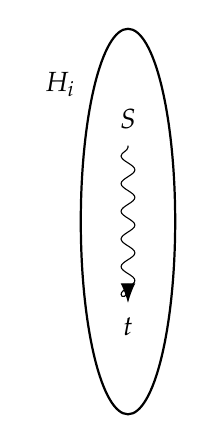
\begin{tikzpicture}[declare function={rr=1+0.1*rnd;}]
        %nodes
        \begin{scope}[every node/.style={circle,thick,draw}]
            \node[draw=none] (S) {$S$};
            \node[draw=none,below = 2cm of S] (t) {$t$};
        
            \node[draw=black,fit=(S)(t) ,inner sep=0.5ex,ellipse] (tmp) {};
            \node[draw=none,left] at (tmp.north west){$H_i$};
        \end{scope}
        
        %crosses
        \begin{scope}
            \tikzset{decoration={snake}} 
            \draw[{Latex[length=2.5mm]}-,decorate] (t)--(S);
        \end{scope}
        \end{tikzpicture}
        \caption{Internal path}
        \end{subfigure}
            \begin{subfigure}[b]{0.49\textwidth}
                \centering
        
        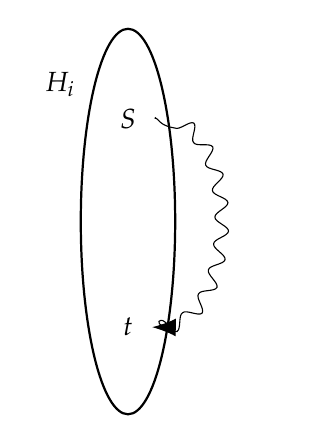
\begin{tikzpicture}[declare function={rr=1+0.1*rnd;}]
        %nodes
        \begin{scope}[every node/.style={circle,thick,draw}]
            \node[draw=none] (S) {$S$};
            \node[draw=none,below = 2cm of S] (t) {$t$};
            \node[draw=none,right = 1.5cm of S] (invis) {};
        
            \node[draw=black,fit=(S)(t) ,inner sep=0.5ex,ellipse] (tmp) {};
            \node[draw=none,left] at (tmp.north west){$H_i$};
        \end{scope}
        
        %crosses
        \begin{scope}
            \tikzset{decoration={snake}} 
            \draw[{Latex[length=3mm]}-,decorate] (t) to [bend right=90](S);
        \end{scope}
        \end{tikzpicture}
        \caption{External path}
        \end{subfigure}
        \caption{The internal pair $(s,t)$ in the house $H_i$ linked internal and linked external}.
        \label{fig:internalpair}
    \end{figure}

    Step 9-11: if $\Pi^e\cup \Pi_1=\emptyset$ , either we have already found all external paths or there is none. 
    Either way, all terminal pairs left are internal hence $\Pi =\Pi_2$. 
    So we are only interested in finding the internal path of the internal pairs, which is why we can call $\mathcal{M}$ on each house for itself.
    Each $K_i$ could be a big graph in itself that is decomposable with at least some house $H_i$ where $|H_i|\geq 2$, if this is not the case the algorithm returns after step 3, and continue with the next. 
    If $\mathcal{M}$ has already found some external paths, $F$ might not be empty  and may use some arcs inside $K_i$ therefore $F\cap A(K_i)$. $\Pi \cap K_i$ is because we are not interested in the terminal pairs that are not a part of the graph we are looking at (pairs inside $K_j$ where $j\neq i$).

    Step 12: Looking for external paths in a big graph is a bit more defficult since we do not know which arcs and vertices not to use.
    
    Step 13-14: First we find all the pairs that are internal pairs, that we want to link as internal paths, the number of these is $k'_i$ for each $i=1,\dots l$. 
    Then we choose a very specific size of vertex sets $W_i$ and loop over every choiche of these.
    This vertex set induces a subdigraph, where we make a possible arc set $F_i$ containg no arcs of $F$.
    We make this set as big as we need to link the external pairs and some internal pairs (those we want to find external paths of $\Pi^e\cup \Pi_1$) the number of those is $k'-k'_i$ since every pair maybe has to go through the house we are looking at.
    
    Step 15-19: For each house, we remove all vertices not in the vertex set $W_i$. 
    After removing these vertices, we remove all remaining arcs except those arcs in $F_i$.
    This is defined in the algorithm as $D''$. We can show that $D''\in \phi(2k^2)$. 
    First we know that since $D$ is totally decomposable $S\in \phi$ and from \autoref{def:bombproof} and the definition of $D(c)$, we can take $S$ and add as many parrallel arcs as we want(no more than a multiplicity of $k$ is needed). 
    We only need to blow up $l$ vertices those houses of $D$ that are not clean we know that there are $k'$ terminal pairs and that $k'\leq k$ meaning $l\leq 2k$ these $l$ vertices needs to be blown up and from \autoref{lemma:external} let us say that we want to find $k''\leq k'$ external paths in $D$ ($|\Pi^e \cup \Pi_1|=k''$). 
    Then we are only looking at $k''$ terminals, meaning in every blow up we need at most $2k''(k''+(k-k'))$. 
    Since $k''\leq k'$ we have $2k''(k''+(k-k'))\leq 2k''k$ vertices in $W_i$ and $2kk''\leq 2kk'\leq 2k^2$, which is the biggest number we will need to blow up the $l$ vertices meaning $c=2k^2$ so $D''\in \phi (2k^2)$.

    Step 20-24: We need to make sure that the tuple $[K_i,k,k'_i,\Pi_2 \cap K_i,F_i\cup(F\cap A(K_i))]$ upholds every condition for every choice of that tuple. 
    Since we are not focusing on loops, we know that the max number of arcs is bounded by the max number of vertices $|F_i|\leq 2kk''$. The rest of the terminals is the number of internal pairs which we in the algorithm denote $k'_i$. we know that $k'_i\leq k'-k''$ meaning $k''\leq k'-k'_i$.
    we start calculating the two demands of $F$ given in the tuple.
    Note that $d_{(F\cap A(K_i))}(v)=d_{F}(v), \ \forall v\in V(K_i)$ and we also know $d_{F_i}(v)\leq k''$ so
    \begin{align}
        d^+_{F\cup F_i},d^-_{F\cup F_i}\leq k-k' + k'' = k-(k'-k'')\leq k- k'_i \\
        |(F \cap A(K_i))\cup F_i|\leq |F|+|F_i|\leq 2k(k-k') +2kk''\\
        \leq 2k(k-\textcolor{blue}{k'})+2k(\textcolor{blue}{k'}-k'_i)=2k(k-k'_i).
    \end{align}
    Clearly the tuple for $F$ holds for all its conditions.

\begin{figure}
    \centering
    \begin{tikzpicture}
        %\draw [help lines] (0,0) grid (4,4);

        \node (t2) {$t_2$};
        \node[draw=red,fit=(t2) ,inner sep=1.3ex,circle] (inner1) {};
        
        \node[below right = of t2] (invis1) {};
        \node[draw=green,fit=(invis1) ,inner sep=2ex,circle] (inner2) {};

        \node[above right = of invis1] (t3) {$t_3$};
        \node[draw=red,fit=(t3) ,inner sep=0.7ex,circle] (inner3) {};

        \node[above = 2cm of t3] (t6) {$t_6$};
        \node[above = of t6] (s6) {$s_6$};
        \node[draw=red,fit=(t6)(s6) ,inner sep=1ex,ellipse] (inner4) {};
        
        \node[above = 2cm of t2] (s3) {$s_3$};
        \node[above = of s3] (blank) { };
        \node[draw=red,fit=(s3)(blank) ,inner sep=2.4ex,ellipse] (inner5) {};

        \node[draw=red,fit=(inner1)(inner2)(inner3)(inner4)(inner5) ,inner sep=1ex,ellipse] (outer1) {};
        \node[draw=none,left] at (outer1.north west){$H_4$};


        \node[right = 4cm of t6] (s5) {$s_5$};
        \node[below right = of s5] (s7) {$s_7$};
        \node[below left = of s7] (t7) {$t_7$};
        \node[draw=red, fit=(s5)(s7)(t7),inner sep=3ex,ellipse] (Outer) {};
        \node[draw=none,left] at (Outer.north west){$H_3$};

        \node[below = 5.2cm of s7] (s8) {$s_8$};
        \node[left = of s8] (t8) {$t_8$};
        \node[draw=red, fit=(t8)(s8), inner sep=0.7ex,ellipse] (inner6) {};
        \node[below = of s8] (invis2) {};
        \node[draw=green, fit=(invis2), inner sep=0.7ex,ellipse] (inner7) {};
        \node[left = of invis2] (invis3) {};
        \node[draw=green, fit=(invis3), inner sep=0.7ex,ellipse] (inner8) {};
        \node[draw=red, fit=(inner6)(inner7)(inner8), inner sep=0.2ex,ellipse] (innerout1) {};
        \node[below left = 2.4cm of t8] (invis4) {};
        \node[left = of invis4] (invis5) {};
        \node[draw=green, fit=(invis4)(invis5), inner sep=2.4ex,ellipse] (innerout2) {};
        \node[draw=red, fit=(innerout1)(innerout2), inner sep=0.5ex,ellipse] (outer2) {};
        \node[draw=none,left] at (outer2.north east){$H_5$};

        \node[above = 4.5cm of s3] (s2) {$s_2$};
        \node[above right = 2cm of s2] (t1) {$t_1$};
        \node[draw=red, fit=(s2)(t1),ellipse] (outer3) {};
        \node[draw=none,left] at (outer3.north west){$H_1$};
        \node[right = 5cm of t1] (s1) {$s_1$};
        \node[below right = 1.5cm of s1] (t4) {$t_4$};
        \node[below left = 1cm of t4] (t5) {$t_5$};
        \node[above left= 0.5cm of t5] (s4) {$s_4$};
        \node[draw=red, fit=(s1)(t4)(t5)(s4), inner sep=0.5ex,ellipse] (outer4) {};
        \node[draw=none,left] at (outer4.north west){$H_2$};
        %\node[below right = of ] (invis1) {$t_3$};
        %\node (t3) {$t_3$};
        %\node[below right = of outer1,draw=red,double,fit=(t3) ,inner sep=1ex,circle] (outer2) {};

        %\node [above right = of none] (z){mussi};
    \end{tikzpicture}
    \caption{Example for the algorithm $\mathcal{M}$. The Figure is a digraph where the red circles is the totally $\phi$-decompostion each house $H_1,H_2,H_3,H_4,H_5$ is either a digraph in $\phi$ ($H_1,H_2,H_3$) or totally $\phi$-decomposable($H_4,H_5$). For $H_4$ the red and green circles inside is the houses of the totally $\phi$-decomposition. Same goes for $H_5$.
    $s_1,\dots ,s_8$ is the source vertices of each terminal pair and $t_1,\dots ,t_8$ are the sink vertices of the terminal pairs. 
    $\Pi=\lbrace (s_1,t_1),\dots ,(s_8,t_8)\rbrace$.}
    \label{fig:mainexample}
\end{figure}
\begin{example}
    This example  is based on \autoref{fig:mainexample}.
    The whole figure is considered one digraph $D$ and the set $\Pi = \lbrace (s_1,t_1),\dots ,(s_8,t_8)\rbrace$.
    $D$ is totally $\phi$-decomposable and contains a $\Pi$-linkage. 
    Step 4 returns the houses that is the outer red circles in the figure. 
    Since the decomposition is not trival, $D'=D$. 
    We look for clean houses for which there are none. So after step 8 we split $\Pi$ up to external pairs $\Pi^e=\lbrace (s_1,t_1),(s_2,t_2),(s_5,t_5)\rbrace$ and internal pairs $\Pi^i=\lbrace (s_3,t_3), (s_4,t_4), (s_6,t_6),(s_7,t_7),(s_8,t_8)\rbrace$. 
    In this example, the partition of the internal pairs are going to be focusing on internal paths before external paths, meaning $\Pi_1=\emptyset$ first, then all set combination of one pair than two pairs and so on.
    So first we have $\Pi_1=\emptyset$ and $\Pi_2=\Pi^i$.
    Since $\Pi^e\cup \Pi_1\neq \emptyset$, we enter the if-statement in step 14. 
    Then we make the vertex sets $W_i$ which we do not go deep into in this example.\\ 
    Let us say that that we succesfully link the external paths and we now call $\mathcal{M}$ recursively on each house starting with the house in the upper left corner.
    Since we have linked the pairs that was present in this house, $\Pi=\emptyset$ and we return. 
    The algorithm now calls itself recursively on the house in the upper right corner.
    Let us say this house $H_2\in \phi$. Since there are two external terminals in house originally $F$ is properly not empty but it does not matter since we call $\mathcal{B}_{\phi}^-$ that accounts for this.
    In this case, $\mathcal{B}_{\phi}^-$ succesfully link the pair $(s_4,t_4)$.  
    The next house will be the one under, let us say that the decomposition of this also is trivial. 
    $\mathcal{B}_{\phi}^-$ can not link $(s_4,t_4)$, meaning the algorithm returns and makes a new partition $\Pi_1=\lbrace (s_3,t_3) \rbrace$ and the rest in $\Pi_2$. 
    Since there is no difference when it comes to the house $H_3$ the algorithm end up returning agian after all the same steps. The algorithm makes a new partition $\Pi_1=\lbrace (s_4,t_4) \rbrace$ and $\Pi_2=\lbrace (s_3,t_3),(s_6,t_6),(s_7,t_7),(s_8,t_8)\rbrace$. 
    All the external pairs are linked including the pair $(s_4,t_4)$. 
    We call the 3 first houses and like before exept now $H_3$ has no terminals that needs to be linked, so we return and continue with the house to the left.\\
    $H_4$ has unlinked terminals and the $\phi$-decomposition is not trivial, we see the houses in \autoref{fig:mainexample}. 
    The green house is a clean house and so is the house contaning $t_2$. 
    Since it is already linked, in step 8 we contract these two sets. 
    In step 9 we split the pairs into external and internal pairs $\Pi^e=\lbrace(s_3,t_3)\rbrace$ and $\Pi^i=\lbrace (s_6,t_6)\rbrace$, so again since $\Pi^e\cup \Pi_1\neq \emptyset$.
    So we enter the if-statement in step 14 link the external pair and then call the algorithm recursively on the houses. 
    Except the houses we have contracted. 
    Either we end up linking the pair as an internal path or we return and link it as an external path. 
    We return all the way to the main digraph and call $\mathcal{M}$ on the last house. \\
    This is not a trival decomposition as there is only an internal pair no external pairs, we contract the green clean house and instead of entering the if-statement in step 14, we enter the if-statement in step 11. 
    In this if-statement we do not have to construct a set of arcs for the external paths since there are none. 
    We directly call $\mathcal{M}$ recursively on the house, there is only one house, and this house does not have a trivial decomposition. 
    Then we contract the two green clean houses and enter the if-statement at step 11, since $\Pi_1=\emptyset$ and $\Pi_2=\lbrace (s_8,t_8)\rbrace$.   
    It turns out that there only is a $(t_8,s_8)$-path but no $(s_8,t_8)$-path so we return and make a new partition  $\Pi_1=\lbrace (s_8,t_8)\rbrace$ and $\Pi_2=\emptyset$ and enter step 14 instead and we end up linking the piar external. \\
    We enter step 27 and return and enter step 27 and return and now we are at the main digraph (the root level). 
    Enter step 27 and output that a linkage exists. 
\end{example}
\begin{proof}
    We have now proven and explained each step in the algorithm, each step does what it is supposed to. 
    Now we need to check whether given your favorite digraph, that upholds the conditions, the algorithm gives the right result.
    If the digraph do not terminate before examining list $\Pi^e\cap \Pi_1$ of $k''$ terminal pairs if $k''=0$ we enter step 9 and $F_i=\emptyset, \text{ for } i=1,\dots l$, and by the induction hypothesis we can assume that if there exists a weak linkage in each $K_i$ the algorithm would find it. 
    Now if this is not the case and $k''>0$, step 12 is then entered and we construct $D''$ which as described belong to $\phi(2k^2)$. then we can use $B_\phi^-$ which is correct by \autoref{def:bombproof}. 
    So the algorithm will find a weak $\Pi''$-linkage if it exists in $D''\backslash F'$. 
    After all this there is made a recursive call on each $K_i$ finding $k'_i$ weak linkages and by the above proof of step 20-24 we know we can and by the induction hypothetise it returns with the linkage.\\ 
    So since $B_\phi^-$ correctly finds the weak linkage inside $D''\backslash F'$ using only arcs from $F_i$ $\forall i\in[l]$, then each $K_i$ is recursively called from $D''$ and do not use any of the arcs in $F_i$ by the induction hypothesis of the algorithm. 
    So we can easily construct to $D'$ from $D''$ since the weak $k'_i$-linkage inside each $K_i$ not using any of the arcs from $F_i$ and the external path do only use the arcs of $F_i$. 
    We know that together these still form the seperated weak linkages.
    By \autoref{lemma:deletarcs} we know that we can find a weak linkage in $D\backslash F$ if we can find it in $D''\backslash F'$ which we just proved we can, 
    returning a perfekt weak $\Pi$-linkage of $D$.\\

    Now we prove that the running time is polynomial.
    Let $T(n,k,k')$ the upper bound running time of the algorithm.
    We assume that $T(n,k,k')$ by induction on $n$ and $k'$ is $O(n^{c(k')})$ for fixed function $c(k')$.
    If $n=0$ time is constant same if $k'=0$.
    Algorithm $\mathcal{A}_\phi$ in step 4 is polynomial from definition and the same is $\mathcal{B}_\phi^-$ in step 6. Contracting the clean houses is also polynomial. Let say that all these steps together takes $O(n^{b(k')})$ for some fixed function $b(k')$.
    All combinations of $\Pi_1,\Pi_2$ is $O(2^k)$ which we see as constant, since $k$ is fixed.
    Step 12: are recursive call on the \autoref{alg:weakphi} hence the time of this step is all the calls $\sum_{i=1}^lT(n,k,k_i')$ with $n_i=|V(K_i)|$. 
    In worst case there are no clean houses so $\sum_{i=1}^ln_i=n$.
    Since we have entered the if-statement in step 11, all terminal pairs are internal and $\sum_{i=1}^lk'_i=k'$.
    By induction hypothesis $\sum_{i=1}^lT(n,k,k_i')$ takes $\sum_{i=1}^lO(n_i^{c(k'_i)})$.\\
    The if-statement in step 14 we choose $W_1,\dots W_l,\ F_1,\dots ,F_l$ combinations of these is at most $\left( {{n}\choose {2k'^2}}\cdot {{4k'^4}\choose {2k'^2}}\right) ^{2k'}$, we will prove that this is the same as $O(n^{4k'^3})$. '
    Since $k'$ is fixed ${{4k'^4}\choose {2k'^2}}$ can be treated as a constant.
    ${{n}\choose {2k^2}}=\frac{n!}{(2k^2)!(n-2k^2)!}$ and we have $\lim_{n\rightarrow \infty}\frac{\frac{n!}{(2k'^2)!(n-2k'^2)!}}{n^2k'^2}=\frac{1}{2k'^2}$ which is a constant so we have that ${{n}\choose {2k'^2}}=O(n^{2k'^2})$.
    Thus
    \begin{align*}
        \left( {{n}\choose {2k'^2}}\cdot {{4k'^4}\choose {2k'^2}}\right) ^{2k'}=\left(O(n^{2k'^2})\right)^{2k'}=O(n^4k'^3).
    \end{align*}
    This is how many times we have to run step 21: which is polynomial by correctness of $\mathcal{B}_\phi^-$ say it takes time $O(n^{d(k')})$ and the recursive calls in step 23: $\sum_{i=1}^lT(n_i,k,k'_i)$. 
    The whole if-statement takes time
    \begin{align}
        O(n^{4k'^3})(\sum_{i=1}^lT(n_i,k,k_i')+O(n^{d(k')})).
    \end{align}
    Now we use the same argument as in the proof of \autoref{thm:philinked} and get 
    \begin{align}
        O(n^{4k'^3})(2k'\cdot T(n,k-1,k'-1)+O(n^{d(k')})).
    \end{align}
    We let $c(k'):=10^{k'}+d(k')+b(k')$ and we will see that both if-statements take at most $O(c^k)$.
    The first if-statement in step 11.
    \begin{align}
        \sum_{i=1}^lO(n_i^{c(k'_i)})=O(\sum_{i=1}^ln_i^{c(k'_i)})=O((\sum_{i=1}^ln_i)^{c(k')})=O(n^{c(k')}).
    \end{align}
    We now make the same calculations for the if-staement in step 14 which takes time at most
    \begin{align}
        O(n^{4k'^3})(2k'\cdot T(n,k-1,k'-1)+O(n^{d(k')}))=O(n^{4k'^3})(O(n^{c(k'-1)})+O(n^{d(k')}))=\\
        O(n^{4k'^3+10^{k'-1}+d(k'-1)+b(k'-1)})+O(n^{4k'^3+d(k')}).
    \end{align}
    We just need these inequalities to hold
    \begin{align}
        4k'^3+10^{k'-1}+d(k'-1)+b(k'-1)\leq 10^{k'}+d(k')+b(k')
    \end{align}
    clearly $d(k-1)+b(k-1)\leq d(k')+b(k)$ left we have $4k^3+10^{k-1} \leq 10^{k'}$ which is obviously also true.
    We also clearly have $d(k)+4k^3\leq c(k')$.
    Thus the whole loop takes at most $O(n^{c(k)})$. (recall that $k'\leq k$ so in worst case which is what we are focusing on $k=k'$).
    And left we have that 
    \begin{align}
        T(n,k,k')\leq O(n^{c(k)})+O(n^b(k))=O(n^c(k)).
    \end{align}
\end{proof}

\subsection{$k$-linkage problem for quasi-transitive digraphs}
We have already established in \autoref{sec:quasi} that quasi-transitive digraphs are totally $\phi_1$-de-\\composable.
It turns out that we just have to prove that $\phi_1$ is bombproof. 
For that we need the two polynomial algorithms $\mathcal{A}_{\phi_1}$ and $\mathcal{B}_{\phi_1}$. Recall that $\phi_1$ is built up by semicomplete and acyclic digraphs so we need to establish some theorems for the weak $k$-linkage problem on semicomplete and acyclic digraphs.
\begin{thm}
    The weak $k$-linkage problem is polynomially solvable for every fixed $k$ when the input is an acyclic digraph.
\end{thm}
\begin{thm}
    The weak $k$-linkage problem is polynomial for every fixed $k$, when we consider digraphs that are obtained from a semicomplete digraph by replacing some arcs with multiple copies of those arcs and adding any number of loops.
\end{thm}

Since the bombproof class allows the digraph to no longer be a part of that class, we need to consider that an acyclic digraph can get a cycle when blowing up a vertex. 
\begin{thm}
    For every natural number $p$, the weak $k$-linkage problem is polynomial for every fixed $k$, when we consider digraphs with most $p$ directed cycles.
    \label{thm:cycleklink}
\end{thm}
% This is a direct consequence of 
%\begin{thm}
%    For every natural number $\theta$ the weak $k$-linkage problem is polynomial for every fixed $k$, when we consider digraphs with cutwidth at most $\theta$.
%\end{thm}

Now we can prove that $\phi_1$ is bombproof and therefore that quasi-transitive digraphs have a polynomial solution for the weak $k$-linkage problem, when $k$ is fixed.

\begin{thm}
    The class $\phi_1$ is bombproof.
    \label{thm:phi1bomb}
\end{thm}
\begin{proof}
    For $\phi_1$ to be bombproof it has to adhere the properties of \autoref{def:bombproof}, the totally $\phi_1$-decomposition can be found in polynomial time for any $\phi_1$-decomposable digraph by \autoref{thm:phipoly}.
    Now we only need the algorithm $\mathcal{B}_{\phi_1}$ for this we need to look at the construction of $D(c)$ where $D\in \phi_1$.
    Let $D'\in D(c)$. 
    Either $D$ is semicomplete or $D$ is acylic.\\
    If $D$ is semicomplete, $D'$ has at most $c$ blown-up vertices $H_1,\dots H_c$ of $D$ to size at most $c$.
    If these $H_i$ are independent, we do not need more then $c^2$ arcs, for each $H_i$ to be semicomplete. 
    So there are at most $c^3$ arcs missing from $D'$ for it to be semicomplete, then by \autoref{lemma:deletarcs}, we can find a weak $k$-linkage for $D'$ if $D$ is semicomplete.
    Now suppose $D$ is an acyclic blowing up $c$ vertices with at a size at most $c$, we have inside these of the acyclic digraph no more than $O(c^c)$ cycles pressent in the house.
    Since $D$ is acyclic there are no cycles between the houses. 
    There are at most $k$ parallel arcs since no more are needed. 
    Which brings up the number of cycles in the house to $O((ck)^c)$ so there are at most $O(c\cdot (ck)^c)$ cycles in $D'$. 
    Then we can use \autoref{thm:cycleklink} where we let $p=c\cdot (ck)^c$.
    So for all possibilities of $D$ and all cases of $D'\in D(c)$ we have a polynomial algorithm that solves the $k$-linkage problem, meaning the $\mathcal{B}_{\phi_1}$ algorithm exists and $\phi_1$ is a bombproof class.
\end{proof}



\section{Solving Weak-Linkgae in Locally Semicomplete Digraphs}
\label{sec:wLocally}
Locally semicomplete digraph can be round-decomposable it turns out that we can from the independece number $\alpha (D)$ tell wether a digraph is round-decomposable or not.
Recall independence number from \autoref{sec:digraph}. The theorem below is from \cite{bangJGT77} where we omits some part of it since we have it statet elsewhere in the thises.
\begin{thm}~\cite{bangJGT77}
    A locally semicomplete digraph $D$ havinng idependece number $\alpha (D)$ at least 3 is round decomposable with a unique round -decomposition. 
    \label{thm:independenceround}
\end{thm} 
This means when considering all other locally semicomplete digraphs it has an independence number $\alpha (D) \leq 2$ which means for all not round-decomposable locally semicomplete digraphs we can use the algorithm in \autoref{thm:independencepoly} to solve the weak $k$-linkage problem when $k$ is fixed.
\begin{thm}
        For every natural number $\alpha$ the weak $k$-linkage problem is polynomial for every fixed $k$, when we consider digraphs with independence number at most $\alpha$.
    \label{thm:independencepoly} 
\end{thm}
For solving the weak $k$-linkage problem in locally semicomplete digraphs we now only need to find a polynomial algorithm for the round-decomposable once.
Before going into this we have to introduce something called the cutwidth. This definition of cutwidth is inspired by the describtion of the cutwidth in \cite{bangJGT77}.\\
Given a digraph $D$ and an ordering of the vertices $O=v_1,\dots,v_n$ we say that the ordering $O$ has a \textbf{cutwidth} at most $\theta$ if $\forall j\in {2,3, \dots n}$ there are at most $\theta$ arcs $u,v$ with $u\in \lbrace v_1,\dots ,v_{j-1}\rbrace$ and $v\in \lbrace v_j,\dots ,v_n\rbrace$ 
\textcolor{red}{inset figur som viser cutwidth $\theta$ for givet ordering}.
Say we have another ordering $O'$of the same digraph $D$, if $O'$ has a cutwidth at most $\theta$ for all possible orderings $O'$ of $D$, then $D$ is said to have a \textbf{cutwidth} at most $\theta$. \\
The minimum natural number $\theta$ such that $D$ has a cutwidth at most $\theta$, we call $\theta$ \textbf{the cutwidth} of $D$.
When we know the cutwidth of the digraph we can solve the weak $k$-linkage problem for those i polynomial time.
\begin{thm}~\cite{bangJGT77}
    For every natural number $\theta$ the weak $k$-linkage problem is polynomial for every fixed $k$, when we consider digraphs with cutwidth at most $\theta$.
    \label{thm:cutwidthklink}
\end{thm}
For the rest of this section  \textbf{interval} will be used with respect to the round ordering of a round digraph. An \textbf{interval} is a subset of vertices $v_iv_{i+1}\dots v_{j-1}v_j$ where the vertices is consecutive compared to the round ordering. In this case the intervals left and right endpoints is $v_i$ and $v_j$ respectively.
From a round digraph $D$ we are going to construct another digraph called the \textbf{compression of $D$ with respect to $\Pi$} and is denoted $D_{\Pi}$. \\
We will Now introduce disjoint intervals $I_1,\dots ,I_l$ where all terminals are containt in there union ($\Pi \subseteq \bigcup_i ^l I_i$) and the left endpoint of each $I_i$ is a terminal.
Also the next $6k$ vertices on the left of the interval $I_i$ are not terminals.
The next $6k$ vertices on the right of the interval are not terminals either this is true for all $i\in [l]$. 
let $I_1$ be the interval which left endpoint is a terminal with the lowest possible number in the round ordering that adhere the properties of the intervals endpoints.
This condition enforces uniqeuness.\\
This can be done unless the digraph is smaller than $12k^2$.
How we find these intervals will be deskribed later in this section.
First we want to introduce $L_i$ and $R_i$ which are both intervals of the round ordering and $L_i$ is the $3k$ vertices left of $I_i$ and $R_i$ is the $3k$ vertices right of $I_i$.
Now we have the rest of the vertices that are not in any interval and we define $W_i$ to be the interval of the vertices between $R_i$ and $L_{i+1}$.
See figure in \cite{bangJGT77} page 103.\\
Now the compression of $D$ with respect to $\Pi$ is the digraph obtaint from $D$ by contracting $W_i$ and if nessesary we delete arcs such that only $k$ multiple arcs is left (the maximum multiplicity of an arc is $k$).

We want to show that finding a weak $\Pi$-linkage in a round digraph $D$ you can just as well find a weak $\Pi$-linkage in its compression with respect to $\Pi$. 
This can only be done for round digraph with cutwidth at least $\Theta =k(6k+36k^2(2k+1)^2)$.
Since the cutwidth is so large we can clearly see that the size of $D$ is not smaller than $12k^2$ so we can construct $D_{\Pi}$.

\begin{lemma}
    Let $D$ be a round digraph with round ordering $O$ and cutwidth at least $\Theta$. 
    Let $\Pi$ be a list of terminal pairs. 
    $D$ has a weak $\Pi$-linkage if and only if its compression with respect to $\Pi$, $D_{\Pi}$, has a weak $\Pi$-linkage.
    \label{lemma:iwanttoprove}
\end{lemma} 

The construction of $D_{\Pi}$ is based on the intervals $I_i$. 
For the first interval $I_1$ we find the first terminal $\tau$ where any of the $6k$ vertices left of $\tau$ are not terminals.
We now make $\tau$ the left endpoint of $I_1$ and look at the $6k$ vertices to the right if they contain another terminal $\tau '$ we let every vertex uptill $\tau '$ including $\tau '$ be in $I_1$ and look right on the next $6k$ vertices from $\tau '$ if it contains a terminal include it in $I_1$ as we did with $\tau '$ if no twe have $I_1$ and we know that the next terminal $\tau *$ right of $I_1$ has at least $6k$ vertices to the left that are not terminals. We now make $\tau *$ the left endpoint of $I_2$ then we do with $I_2$ as we did with $I_1$.
We keep doing this untill all terminals is a part of an interval $I_i$.
Then we can easily construct $L_i$ and $R_i$ from $I_i$ and from this we can find $W_i$ if it exists (is not empty) do this forall $i\in [l]$. then we constract $W_i$ and we now have constructed $D_\Pi$. \\
In this thesis we are focusing on the decomposable digraphs and we can define a compression for the round decomposable digraphs too. As the compression for round digraphs the compression of round decomposable digraphs is both defined in $\cite{bangJGT77}$ page 102 - 105.
So we assume $D=R[H_1,\dots ,H_r]$ is round decomposable. 
Then we contract the clean houses so we now have $D'=R'[H'_1,\dots ,H'_r]$ which is the digraph after the contraction. 
The only difference between $R'$ and $R$ is the multiplicity of the arcs, we will construct $\Pi '$ from $\Pi$ where for each pair, $(s_i,t_i)\in \Pi$ where $s_i\in H_z$ and $t_i\in H_q$, we make a pair $(v_z,v_q)\in \Pi'$ where $v_z,v_q\in V(R')$.
We now make a compression of $R'$ with respect to $\Pi'$, $R'_{\Pi'}$. 
Let $v_{j_1},\dots ,v_{j_p}$ be the vertices of the compression $R_{\Pi'}$.\\
Now we define the compression of $D$ with respect to $\Pi$ to be the digraph $D\Pi=R'_{\Pi'}[H'_{j_1},\dots ,H'_{j_p}]$.
The intervals $I_j$ are the only once with terminals in and therefore the only intervals of $R'_{\Pi'}$ that have some blown-up vertices in $D_\Pi$.
We know from $\autoref{lemma:cleanhouse}$ that we can contract the clean houses and in the prove of \autoref{lemma:iwanttoprove}, which can be found in $\cite{bangjgt77}$ page 103-104, that the path are split up in $(s_i,\sigma _i)$-path, $(\sigma_i,\tau_i)$-path $(\tau_i,t_i)$-path that obviouse joined together is an $(s_i,t_i)$-path. 
The $(\sigma_i,\tau_i)$-path is not inside any $I_b$ interval and follow therefore by lemma 5.5 in \cite{bangJGT77}. 
Both the $(s_i, \sigma_i)$-path and the $(\tau_i,t_i)$-pathdo not use the property of $I_b$ being round and can therefore be linked in the same way for $D_\Pi=R'_{\Pi'}[H'_{j_1},\dots ,H'_{j_p}]$. 
Which brings us to this lemma.
\begin{lemma}
    Let $D$ be a digraph of the form $D=R[H_1,\dots H_r]$, where $R$ is round and has cutwidth at least $\Theta$. Let $\Pi$ be a list of piars of terminals. $D$ has a $\Pi$-linkage if and only if $D_\Pi$, has a $\Pi$-linkage.
    \label{lemma:compressiondecom}
\end{lemma}
Now we can use all this to prove that $\phi_2$ which is defined in \autoref{sec:gdecomposable} is bombproof and recall that round-decomposable digraphs is totally $\phi_2$-decomposable.
\begin{lemma}
    The class $\phi_2$ is bombproof
\end{lemma}
\begin{proof}
    For $\phi_2$ to be bombproof we need to find $\mathcal{A}_{\phi_2}$ which we have from \autoref{lemma:phipoly}.
    we have already proven the existens of $\mathcal{B}_{\phi_2}$ if $R\in\phi_2$ is semicomplete for this see the prove of \autoref{thm:phi1bomb}.
    Therefore assume that $R$ is round we  want to show that the weak $k$-linkage problem is polynomial on $R(c)$ for a positive integer $c$.
    Let a digraph $D\in R(c)$. Now recall $\Theta = k(6k+36k^2(2k+1))^2$ then when $R$ is round we will base the prove on two cases one where $R$ has a cutwidth at least $\Theta$ and another where $R$ has cutwidth at most $\Theta$.\\
    In both cases we have $D=R[H_1,\dots ,H_r]$ where at most $c$ of the $H_i$ houses has $|V(H_i)|>1$ and $R$ has an ordering $O$, $v_1,\dots ,v_r$ where $H_i$ in $D$ corresponds to $v_i$ in $R$.
    \begin{itemize}
        \item[Case 1] When a digraph $D=R[H_1,\dots ,H_r]$ with size $|V(R)|\geq 12k^2$ we can create a compression of $R$ with respect to some $\Pi*$ created from $\Pi$, and therefore we can construct the compression of $D$ with respect to $\Pi$, $D_{\Pi}$.
        As we know from the way we constructed $D_\Pi$ the size is only depending on $c$ and $k$, since $R_{\Pi*}$ is has a size depending on $|\Pi*|\leq k$ and we blow up at most $k$ vertices to a size at most $c$. 
        Since $c$ and $k$ are both fixed naturel numbers we use a brute-force algorithm (an algorithm that checks all possibilities) to solve the weak $\Pi$-linkage problem on $D_\Pi$ and from \autoref{lemma:compressiondecom} $D$ has a weak $\Pi$-linkage if and only if $D_\Pi$ has a weak $\Pi$-linkage.\\
        Since $c$ and $k$ are fixed the brute-force algorithm is polynomial and the construction of $D_\Pi$ is also polynomial.
        \item[Case 2] $R$ has a cutwidth at most $\Theta$ for the round ordring $O$ so for $D=R[H_1,\dots ,H_r]$ we construct an ordering $O'$ where for every $u\in H_i$ and $z\in H_j$ with $i\neq j$ we have that $u < z$ in $O'$ if $v_i < v_j$ in $O$.
        The ordering of the vertices inside a house $H_l$ is not important for the prove.
        Now cutwidth $\theta'$ of $O'$ is at most $k(c^3+c^2\cdot \Theta)$.
        To calculate this we know that there is at most $c$ houses $H_i$ where $|V(H_i)|>1$ these houses has size at most $c$. 
        There is at most $c^2$ arcs inside a house with possible multiplicity $k$ since we are not interested in more. So for arcs inside the houses that can contribute to the cutwidth is $c^2\cdot k\cdot c$.
        The other arc that can contribute to the cutwidth $\theta'$ is the arcs between the houses $H_i$ and $H_j$ where $v_i<v_j$ in $O$. 
        The arcs between two such given houses is $c\cdot c\cdot k$ since both has a size on maximum $c$ and the multiplicity of these arcs is at most $k$ we can not find more than $\Theta$ cases of such two houses since they represent vertices of $R$ with cutwidth at most $\Theta$.
        So $\theta'\leq c^3\cdot k+c^2\cdot \Theta \cdot k=k(c^3+c^2\cdot \Theta)$.
        Therefore we can use the algorithm from \autoref{thm:cutwidthklink} to solve the $k$-linkage problem of $D=R[H_1,\dots ,H_r]$ ($R(c)$).
    \end{itemize}
    Thus we have found $\mathcal{B}_{\phi_2}$.
\end{proof}
As mensioned above and proved in \autoref{sec:locally} round-decomposable digraphs is totally $\phi_2$-decomposable and we have just proved that $\phi_2$ is bombproof so by the algortihm \autoref{alg:weakphi} for bombproof classes every round-decomposable digraph now have a polynomial algorithm to solve the weak $k$-linkage problem.
\begin{thm}
    For every fixed $k$ there exists a polynomial algorithm for the weak $k$-linkage problem for round-decomposable digraphs.
\end{thm}
This ends the part for round-decomposable digraph and in the begining of this section we proved that all other locally semicomplete digraphs than the round-decomposable once have a polynomial algorithm for the weak $k$-linkage problem. We can now state this.
\begin{thm}
    For every fixed $k$ there exists a polynomial algorithm for the weak $k$-linkage problem for locally semicomplete digraphs.
\end{thm}


	\clearpage
	%\part{Spanning disjoint subdigraphs (Arc decomposition)}
	%\chapter{strong spanning subdigraphs}
\textcolor{red}{blablabalbalaba}
\section{Arc-decomposition Problem}
\label{sec:garcdecom}
First we need to esablish that a spanning subdigraph of a digraph $D$ is a subdigraph $D'\subseteq D$ contaning all the vertices of $D$.
Finding two such subdigraphs in the same graph that are arc disjoint and strong, this is the problem that we are going to cover.
The problem is NP-complete and this is shown by use of the hamilton cycle problem.
Recall from \autoref{sec:class} a k-arc-strong digraph is a digraph where we need to delete at least $k$ arcs before the digraph is no longer strong. 
From this it is clear that for these two subdigraphs to be present in a digraph $D$, it needs to be 2-arc-strong.
We are going to denote these two subdigraphs as $D_1$ and $D_2$ with the arc set $A_1\subseteq A$ and $A_2\subseteq A$ respectively.
\begin{thm}
    \textcolor{red}{NP-complete blablablabalba}
\end{thm}
\begin{proof}
    \textcolor{red}{sketz blablabalal}
\end{proof}
We are as we have through the whole thises focused on decomposable digraphs, we are in this chapter going to focus more on using the word composition so it is not confusing since we are looking at when there exists an arc-decomposition in a decomposable digraph.

\clearpage

\section{Arc-decomposition in Quasi-transitive digraphs}
\label{sec:arcquasi}
When we talk about quasi-transitive digraphs we know that it is composed from either a semicomplete digraph or an acyclic transitive digraph depending if it is strong or non-strong respectively.
Since we need it to be 2-arc-strong we do not focus on the non-strong quasi-transitive digraphs, which means we have to compose the quasi-transitive digraph from a semicomplete digraph. 
So we are going to estabilsh some results for this problem on semicomplete digraphs.
\begin{thm}~\cite{bangjgt}
    A 2-arc-strong semicomplete digraph $D=(V,A)$ has a arc-decomposition $A_1,A_2$ where both $D_1=(V,A_1)$ and $D_2=(V,A_2)$ are strong digraphs if abd only if $D$ is not isomorphic to $S_4$, where $S_4$ is obtained from the complete digraph with four vertices by deleting the arcs of a cycle of length four. Furthermore, this decomposition can be obtainted in polynomial time when it exists. 
\end{thm}
We have a very semilar theorem for a strong composition of the semicomplete digraphs which is among others the quasi-transitive digraphs.
\begin{thm}
    Let S be a strong semicomplete digraph on $s\geq 2$ vertices and let $H_1,\dots ,H_s$be arbitrary digraphs, each with at least two vertices. Then $D=S[H_1,\dots ,H_s]$ has a strong arc decomposition if and only if $D$ is not isomorphic to one of the following three digraphs: $\overrightarrow{C}_3[\overline{K}_2,\overline{K}_2,\overline{K}_2]$, $\overrightarrow{C}_3[\overline{K}_2,\overline{K}_2,\overrightarrow{P}_2]$, and $\overrightarrow{C}_3[\overline{K}_2,\overline{K}_2]\overline{K}_3$.
\end{thm}
\textcolor{red}{Figur of 3 digraphs above}

\clearpage

\section{Arc-decomposition in locally semicomplete digraphs}
\label{sec:arclocally}
blablabalblabla
\clearpage
	\clearpage
	\section{Conclusions and further results}
	In \autoref{chap:Hamilton} we explored the problem of the hamiltonian cycle and path problem.
	For the locally semicomplete digraphs we did not need to exploit the structure of the decomposability.
	It was shown that the decomposability was of great importance in quasi transitive digraphs, because that the houses' path cover had a correlation to the cycle in the quotient digraph.

	After which, we then explored the linkage problem in \autoref{chap:linkage}, for which we explored an algorithm which was generally applicable to the class of problems that are linkage ejectors.
	$\phi_1$ and $\phi_2$ are both linkage ejectors, such that the problems could be solved for quasi transitive and round decomposable digraphs.
	Since evilly semicomplete digraphs have a semicomplete decomposition of at most three houses, then by \autoref{thm:inducesemi}.

	Finally, in \autoref{chap:weak} we find an algorithm similar to the one used for the linkage problem, with the difference being that the class now must be bombproof.
	$\phi_1$ and $\phi_2$ are bombproof classes, such that we have a solution for both quasi transitive digraphs and round decomposable digraphs.
	Here we solve the rest of the locally semicomplete digraphs that are not decomposable, by utilizing their independence number, which is at most two such that we can apply \autoref{thm:independencepoly}, to solve the weak $k$-linkage problem.

	\subsection{Further results}
	As we have seen throughout this thesis, the structure of decomposable digraphs can be used to solve various problems.
	A problem that would have been of interest to include in this thesis is the arc disjoint strong spanning subdigraphs.
	Bang-Jensen, Gutin and Yeo proved that the arc disjoint strong spanning subdigraphs is polynomially solvable for quasi transitive digraphs in~\cite{bangJGT95}.
	The technique used in~\cite{bangJGT95} is coloring the arcs in two colors, red and blue, which turns out to be the arc decomposition of the digraph $D = (V,A)$.
	\begin{thm}\label{thm:mainresult}
		Let $T$ be a strong semicomplete digraph on $t \geq 2$ vertices and let $H_1, \dots ,H_t$ be arbitary digraphs.
		Then $D = T[H_1, \dots, H_t]$ has a strong arc decomposition if and oly if $D$ is 2-arc-string and is not simorphic to one of the following four digraphs: $S_4,\overrightarrow{C}_3[\overline{K}_2,\overline{K}_2,\overline{K}_2],\overrightarrow{C}_3[\overline{K}_2,\overline{K}_2,\overline{P}_2]$ and $\overrightarrow{C}_3[\overline{K}_2,\overline{K}_2,\overline{K}_3]$.
	\end{thm}
	Since a strong quasi transitive digraph is decomposable where quotient digraph is a semicomplete digraph, \autoref{thm:mainresult} can be used on quasi transitive digraphs.
	\begin{thm}\label{thm:dependent}
		Let $D = T[H_1, \dots, H_t]$ be 2-arc-strong ($t \geq 2$) where T is a semicomplete digraph and every $H_i$ is an arbitary digraph. Then at lease one of the following cases holds.
		\begin{itemize}
			\item[(a)] $D$ has a strong arc decomposition.
			\item[(b)] $D$ is an extended semicomplete digraph.
			\item[(c)] For every $i \in [t]$ and eveyr arc $d$ of $H_i$, $D - e$ is 2-arc-strong.
		\end{itemize}
	\end{thm}
	The main result in~\cite{bangJGT95} is \autoref{thm:mainresult}, which build on \autoref{thm:dependent}.

	The problem is also explored for locally semicomplete digraphs by Bang-Jensen and Huang in~\cite{bangJCT102}.
	\begin{thm}\label{thm:secondpower}
		A 2-arc-strong locally semicomplete digraph $D$ has a good decomposition if and only if $D$ is not the second power of an even cycle.
	\end{thm}
	The proof of \autoref{thm:secondpower} exploits the structure of the evil digraphs described in \autoref{sec:locally}.
\bibliographystyle{unsrt}
\bibliography{bib}
\end{document}